\documentclass[oneside]{ausarbeitung}
\addbibresource{latexlit.bib}
\usepackage{todonotes} 
\usepackage{hyperref}
\usepackage{graphicx}
\usepackage{float}
\hypersetup{draft}

% ----------------------------------------------------------------------

\begin{document}

%--- Sprachauswahl
% Erlaubte Werte:
%   \selectlanguage{english}
%   \selectlanguage{ngerman}
\selectlanguage{ngerman}

%--- Art der Arbeit
% Erlaubte Werte:
%   \Praxissemesterbericht
%   \Projektbericht
%   \Bachelorarbeit
%   \Seminararbeit
%   \Masterarbeit

\Bachelorarbeit

%--- Studiengang:
% Erlaubte Werte:
%   \Informatik
%   \Elektronik
%   \DataScience
\Informatik
\title{Component-Based Web Development: Eine Revolution in der Wiederverwendbarkeit von Webkomponenten?}

\author{Jonathan Kechter}
\matrikelnr{83701}

%--- Ist der Erstbetreuer (\examinerA) an der Hochschule ein Professor?
% Erlaubte Werte:
%   \examinerIsAProfessortrue   % Ja
%   \examinerIsAProfessorfalse  % Nein
\examinerIsAProfessortrue   % Ja

%--- Betreuer
\examinerA{Prof. Dr. Carsten Lecon}
\examinerB{Sebastian Stigler}

%--- Einreichungsdatum
\date{02. April 2025}

%--- Angaben zur Firma
% Auskommentieren, wenn die Arbeit nicht bei einer ext. Firma gemacht wurde.


%--- Angaben zum Betreuer bei dieser Firma


%--- Titelseite Anzeigen
\maketitle
\cleardoublepage

%---
\pagenumbering{roman}
\setcounter{page}{1}

%--- Firmendaten Anzeigen
% Auskommentieren, wenn die Arbeit nicht bei einer ext. Firma gemacht wurde.
%\makeworkplace
\cleardoublepage

%--- Eidesstattliche Erklärung anzeigen
\makeaffirmation
\cleardoublepage

%--- Sperrvermerk (Funktioniert nur bei externen Bachelor- oder Masterarbeiten.)
%\makeconfidentialclause
\cleardoublepage

%---
\begin{abstract}
  Ziel der Kurzfassung ist es, einen (eiligen) Leser zu informieren, so 
  dass dieser entscheiden kann, ob der Bericht für ihn hilfreich ist oder 
  nicht (neudeutsch: Management Summary). Die Kurzfassung gibt daher eine 
  kurze Darstellung

  \begin{itemize}
    \item des in der Arbeit angegangenen Problems
    \item der verwendeten Methode(n)
    \item des in der Arbeit erzielten Fortschritts.
  \end{itemize}

  Dabei sollte nicht auf die Struktur der Arbeit eingegangen werden, also 
  Kapitel~\ref{cha:grundlagen} etc. denn die Kurzfassung soll ja gerade 
  das Wichtigste der Arbeit vermitteln, ohne dass diese gelesen werden muss.
  Eine Kapitelbezogene Darstellung sollte sich in Kapitel~%
  \ref{cha:einleitung} unter Vorgehen befinden.

  Länge: Maximal 1 Seite.
\end{abstract}
%-----------------------------------------------------------------------
\cleardoublepage
\tableofcontents

%---
\listoffigures

%---
\listoftables

%---
\lstlistoflistings

%---
\listofabbreviations
\begin{acronym}[Bsp.]  % Längstes Kürzel in der nachfolgenden
                       % Liste um die Breite der Spalte für die
                       % Abkürzungen zu bestimmen.

%% Eintrag: \acro{Referenzname}[Kürzel]{Langform}
%% Im Text wird die Abkürzung dann mit \ac{Referenzname} benutzt.
\acro{rup}[RUP]{Rational Unified Process}
%\acro{bsp}[Bsp.]{Beispiel}
\end{acronym}
%---


\cleardoublepage
\pagenumbering{arabic}
\setcounter{page}{1}

% ----------------------------------------------------------------------
\chapter{Einleitung}
\label{cha:einleitung}

\section{Motivation}
\label{sec:motivation}

Meine Motivation entstand ursprünglich aus meinem über das Studium hinweg angesammelten Interesse für Web-Technologien. In meinem bisherigen Werdegang habe ich hauptsächlich mit Angular gearbeitet und konnte dort Vorteile und Schwächen der Technologie kennenlernen. Bei zeitweise schlechter Performance treten gelegentlich Zweifel über die Wahl des richtigen Frameworks auf und ein Interesse, ob andere Lösungen wie React, Vue oder Web Components in solchen Fällen effizienter wären. Bei ersten Recherchen findet man schnell die positive Perspektive aus Sicht der Autoren. Was häufig fehlt, ist ein umfassender Vergleich aus verschiedensten Perspektiven.

Bei der Nutzung von neuen Web-Technologien bestand eine gewisse Hürde, diese für neue Projekte ohne Vorkenntnisse zu nutzen, da ein Verständnis über die Vor- und Nachteile der verschiedenen Lösungen fehlte. Mithilfe einer praxisnahen Erfahrung, in der das im Studium erlangte Wissen verwendet werden kann, soll ein umfassender Vergleich anderer Frontendlösungen ermöglicht werden. Durch diese praxisnahe Auseinandersetzung können theoretische und praktische Erfahrungen gesammelt werden, die in zukünftigen Projekten für die Wahl der optimalen Frontendlösung hilfreich sein könnten.

\section{Ursprünge}
\label{sec:ursprünge}

Die Ursprünge der Webentwicklung gehen auf Tim Berners-Lee zurück, der 1991 HTML, HTTP und den ersten Webbrowser entwickelte \parencite{cern-www}. Damit entstand das Web 1.0, das rein statisch war.
Schon bald wurde deutlich, dass rein statische HTML-Seiten nicht ausreichten, um interaktive Inhalte bereitzustellen. So entstand das Web 2.0, das sich durch Interaktivität, Dynamik und nutzergenerierte Inhalte auszeichnete. In diesem Kontext entwickelte sich JavaScript zu einer der zentralen Technologien. JavaScript ermöglichte erstmals, Webseiten interaktiv zu gestalten, etwa durch DOM-Manipulation, Ereignisverarbeitung oder Formularvalidierungen \parencite{js-history}.
Parallel dazu wurde mit CSS eine Sprache eingeführt, die das Ziel hatte, den Inhalt und dessen Darstellung voneinander zu trennen. Durch die Verwendung von CSS konnten erstmals Layouts, Farben und Typografie unabhängig vom eigentlichen HTML-Code gestaltet werden, was ein wichtiger Schritt hin zu wartbaren und visuell ansprechenden Webanwendungen war \parencite{w3c_css_history}. Trotz der Verwendung von JavaScript für die Webentwicklung blieben viele Webpages eine lange Zeit seitenbasiert, wodurch jede Aktion, die mit einer HTTP-Anfrage verbunden war, einen Reload der Seite erforderte. Dies führte zu ineffizienten Ladezeiten und einer unterbrochenen Benutzererfahrung. Um solche Probleme zu lösen, wurden neue Techniken entwickelt, die eine effizientere Datenübertragung ermöglichten. 

AJAX (Asynchronous JavaScript and XML) ermöglichte es erstmals, HTTP-Anfragen durchzuführen, während eine HTML-Seite dargestellt wurde, sodass die Seite aktualisiert werden konnte, ohne sie neu zu laden \parencite{ajax-msdn}. Ein frühes Beispiel für die erfolgreiche Nutzung von AJAX ist die Beta-Version von Google Maps. Hierbei wurden Kartenausschnitte beim Ziehen der Maus nahtlos nachgeladen wurden, ohne dass die Seite neu geladen werden musste, was zu einer erhöhten Performance führte. Auch Gmail setzte auf diese Technik, um eine flüssige Benutzererfahrung mit sofortiger Reaktion auf Eingaben zu ermöglichen \parencite{paulson2005ajax}.

Ein weiteres Tool, das an Popularität gewann, war jQuery. jQuery ermöglicht die Erstellung einer vereinfachten und browserübergreifenden einheitlichen Schnittstelle zur DOM-Manipulation und zum Event-Handling \parencite{taft2006jquery}. jQuery stellt zudem Funktionen bereit, die viele Zeilen JavaScript auf eine einzelne Methode kürzte und somit an Komplexität einsparte. Dadurch wurde es eine beliebte Lösung um komplexe Aufgaben aus JavaScript wie AJAX Calls oder DOM Manipulationen zu handhaben. \parencite{w3schoolsJquery}.

Mit der zunehmenden Komplexität moderner Webanwendungen entstanden ab den 2010er Jahren zahlreiche JavaScript-Frameworks, die den Entwicklungsprozess vereinheitlichen und vereinfachen sollten. 
Eines dieser war AngularJS, ein Framework, das eine MVC-ähnliche Architektur für dynamische Single-Page-Anwendungen bot. Im Gegensatz zu einer Bibliothek welche nur Werkzeuge zur  bietet war Angular das erste Framework, welches auch eine Struktur speziell für Single Page Applications vorgibt. Angular übernimmt Aufgaben wie DOM- und AJAX-Verwaltung automatisch und bietet eine strukturierte Trennung durch das MVC-ähnliche Konzept, das Präsentationslogik (View) und Datenlogik (Model) voneinander trennt. Dies führt zu einer besseren Wartbarkeit, Wiederverwendbarkeit und Testbarkeit von Code \parencite{what-is-angularjs}. Angularjs unterstüzt beispielsweise das Two-Way Data Binding, das Datenfluss zwischen den Model und View automatischt synchronisiert. Außerdem können Formulare mit Validierung in die Applikation eingebunden werden, aber auch Routing, Dependency Injection sowie modulare, wiederverwendbare Komponenten können von Angular gehandhabt werden \parencite{angular-history}. 


Ein weiteres Framework, das in der Web-Entwicklung zum Einsatz kommt, ist React. Im Jahr 2013 von Facebook eingeführt, sollte React das Problem ineffizienter UI-Updates lösen. Durch die Einführung eines virtuellen DOMs und der sogenannten Reconciliation konnte React die Performance bei Änderungen an der Benutzeroberfläche deutlich verbessern \parencite{hunt2013react}.

Heutzutage gehört React neben Angular und Vue.js zuden drei meist verbeiteten Frontend-Frameworks. Vue.js wurde 2015 als leichtgewichtige Alternative zu AngularJS und React entwickelt und verfolgte einen kombinierten Ansatz. 
Es setzte auf eine einfache API, deklarative Syntax und eine reaktive Datenbindung, um eine flexible und effiziente Entwicklung zu ermöglichen \parencite{vue-intro}. 

Angular Version 2 ging auf alte Probleme ein und entwickelte ein neues, komponentenbasiertes Architekturmodell, welches sich in Komponenten, Services und Dependency Injection aufteilte \parencite{angular-docs}. 

Im Jahr 2018 wurden Web Components als offizielle, standardisierte, frameworkunabhängige Lösung für wiederverwendbare Komponenten eingeführt \parencite{mdn-webcomponents}. 
Zudem stellte Svelte im darauffolgenden Jahr mit seinem neuen Konzept eines kompilierten Codes anstelle des virtuellen DOMs einen neuen Ansatz vor \parencite{svelte-intro}.


\section{Problemstellung}
\label{sec:problemstellung}

In der modernen Webentwicklung gibt es zahlreiche Tools, Frameworks und Bibliotheken, die Entwickler bei der Erstellung von Webanwendung unterstützen. Komponentenbasierte Frameworks wie Angular, React und Vue.js heben sich durch ihre Modularität und Wiederverwendbarkeit von Komponenten hervor. Gleichzeitig bringen sie aber auch einige Herausforderungen mit sich. Hierzu zählt beispielsweise ein erhöhter Overhead, komplexere Buildprozesse und größere Bundle-Größen, die sich auf die Performance und Entwicklungsdauer auswirken können.
Gleichzeitig gibt es auch nicht komponentenorientierte Lösungen wie z.B. jQuery, welche durch ihre Einfachheit einen geringeren Entwicklungsaufwand benötigen, dadurch aber weniger skalierbar und modular sind. 
Eine richtige technologische Entscheidung, abhängig von den eigenen Bedürfnissen, bzw. denen des gewünschten Projekts, zu treffen, ist nicht einfach, da ein grundlegender Vergleich zwischen komponentenbasierten Ansätzen und den herkömmlichen Ansätzen fehlt. Vorhandene Vergleiche sind oft aus ungenügend Blickwinkeln durchgeführt worden, sondern beschränkten sich auf Teilaspekte, wie die Performance, Wartbarkeit oder Skalierbarkeit, welche für eine Entscheidung der Frontendtechnologie nicht als einzige Metrik dienen sollte. 

\section{Abgrenzung}
Um die eben beschriebenen Einschränkungen abwägen zu können, sollen in der vorliegenden Forschungsarbeit die Vor- und Nachteile von modernen komponentenbasierten Frameworks gegenüber von klassischen Ansätzen vergleichen zu können, fokussiert sich diese Arbeit auf die Analyse von Frontendtechnologien. 
Die Arbeit wird anhand eines festgelegten Implementierungsbeispiels durch die Verwendung bestimmter Metriken verglichen, was dem Zweck einer einheitlichen Grundlagen dienen soll. Hierbei wird mit folgenden Metriken gearbeitet: 
\begin{itemize}
    \item \textbf{Modularität und Wiederverwendbarkeit}:  
Wie gut lassen sich einzelne Komponenten entwerfen, strukturieren und in unterschiedlichen Projekten wiederverwenden? Dabei wird zudem untersucht, wie effektiv sich User Interfaces von Webseiten unter Verwendung der komponentenbasierten Softwareentwicklung im Hinblick auf Modularität und Wiederverwendbarkeit umsetzen lassen.
    \item \textbf{Performance und Effizienz}:  
          Wie wirken sich Frameworks auf Ladezeiten, Bundle-Größen und Rendering- Geschwindigkeiten aus?
          Welche Mechanismen zur Optimierung (z.\,B. Lazy Loading, Virtual DOM, Compiler) kommen zum Einsatz?
    \item \textbf{Entwicklungsaufwand und Wartbarkeit}:  
          Welche Frameworks ermöglichen eine effiziente und nachhaltige Entwicklung?
                    Wie einfach und intuitiv lassen sich mit dem Framework funktionale Webanwendungen erstellen?
          Wird eine saubere Architektur unterstützt (z.\,B. durch klare Projektstruktur, Type Safety und Tooling)?
\end{itemize}

Nicht Bestandteil dieser Arbeit sind folgende Aspekte: 
\begin{itemize}
    \item \textbf{Backend-Technologien und serverseitige Frameworks}:  
          Technologien wie Next.js, Nuxt.js oder Server-Side Rendering ermöglichen die serverseitige Verarbeitung und Darstellung von Webseiten.  
          Der Fokus dieser Arbeit liegt auf Frontend-Technologien. Serverseitige Lösungen werden nicht betrachtet.
    \item \textbf{State-Management-Lösungen innerhalb der Frameworks}:            Externe State-Management-Bibliotheken wie Redux, NgRx oder Vuex werden nicht 			          untersucht, da der Schwerpunkt auf den komponentenbasieren Entwicklungsaspekt der jeweiligen Frameworks liegt.
    \item \textbf{Full-Stack-Architekturen}:  
          Der Einfluss einer Full-Stack-Architektur auf die Wahl des Frontend-Frameworks wird ebenso nicht analysiert. Die betrachteten Frontend-Technologien werden isoliert betrachtet.
    \item \textbf{Skalierung auf Großprojekte}:  
          Die Anwendbarkeit der Technologien auf groß angelegte Projekte wird nicht untersucht. Eine Performance-Analyse für eine große Anzahl an Nutzern erfolgt nicht.
\end{itemize}

\section{Ziel der Arbeit}
\label{sec:ziel}

Der Vergleich wird anhand verschiedener Metriken erstellt, die unterschiedliche Aspekte der Frameworks beleuchten. Dabei wird zunächst untersucht, wie gut sich Komponenten im jeweiligen Framework erstellen lassen und inwiefern sie innerhalb der Anwendung wiederverwendet werden können, um eine modulare Architektur zu fördern und gleichzeitig Code-Dopplungen zu vermeiden. Darüber hinaus spielt die Performance eine zentrale Rolle, insbesondere hinsichtlich der Ladezeiten, Bundle-Größen und Rendering-Geschwindigkeit. Zusätzlich wird geprüft, ob der Overhead des jeweiligen Frameworks die Performance signifikant beeinträchtigt. Ein weiterer wichtiger Aspekt ist der Entwicklungsaufwand, sowie die Wartbarkeit und Erweiterbarkeit der Frameworks. Es wird analysiert, welche Frameworks eine effiziente und nachhaltige Entwicklung ermöglichen und ob Anwendungen leicht erweitert werden können, indem neue Funktionen hinzugefügt oder bestehende Module angepasst werden. Abschließend wird untersucht, ob die Architektur der Frameworks für größere Nutzerzahlen skalierbar ist und komplexere Anwendungen unterstützt.

\section{Vorgehen}
\label{sec:vorgehen}

Das Vorgehen der Arbeit ist in mehrere strukturierte Abschnitte unterteilt, die in den folgenden Kapiteln behandelt werden. Hierbei wird auf Basis der Grundlagen und der vorgestellten Problemstellung gezielt auf die Lösung hingearbeitet. 
Das komplette Vorgehen lässt sich in folgende Kapitel aufteilen: 

\begin{enumerate}  
\item \textbf{Grundlagen Kapitel 2}: Hier wird auf alle relevanten technischen und theoretischen Konzepte der Arbeit eingegangen um einen gleichen Wissensstand zu garantieren. Das Kapitel befasst sich mit den für die Forschungsarbeit wichtigen Werkzeugen, Grundlagen, Frontendtechnologien sowie mit den Backendtechnologien und dient dazu, ein grundlegendes Verständnis für die folgenden Kapitel zu schaffen. 
    
\item \textbf{Problemanalyse (Kapitel 3)}: In diesem Kapitel wird die aktuelle Situation der Webentwicklung detailliert beschrieben und bestehende Herausforderungen sowie Einschränkungen analysiert. Besonders detailliert wird hierbei betrachtet, wie die unterschiedlichen Ansätzen der Frameworks hinsichtlich Skalierbarkeit, Performance, Modularität, Wiederverwendbarkeit und Wartbarkeit sind. Die identifizierten Probleme dienen als Ausgangspunkt für die Entwicklung des Lösungskonzept sowie die Identifizierung der in der Evaluierung betrachteten Metriken.

\item \textbf{Lösungskonzept (Kapitel 4)}: Auf Basis der zuvor identifizierten Probleme wird ein Lösungskonzept entwickelt, das einen strukturierten Vergleich der Frameworks ermöglicht. Hierbei werden relevante Kriterien wie Modularität, Performance, Entwicklungsaufwand, Skalierbarkeit, Wartbarkeit und State-Management definiert. Zudem wird beschrieben, wie diese Metriken im Rahmen der Implementierung untersucht, gemessen und ausgewertet werden sollen.

\item \textbf{Implementierung (Kapitel 5)}: Dieses Kapitel beschreibt die praktische Umsetzung des Vergleichsansatzes. Dazu wird ein zentralisiertes Backend mit Supabase aufgebaut, welches von mehreren Frontend-Anwendungen (Angular, React, Vue.js, Svelte und jQuery) genutzt wird. Die Implementierung umfasst dabei die Entwicklung von Authentifizierungsmethoden, Produktdarstellungen, Warenkorbfunktionen sowie einen Checkout-Prozess. Jede Frontend-Variante wird separat implementiert und im Anschluss hinsichtlich der definierten Kriterien evaluiert.

\item \textbf{Inbetriebnahme (Kapitel 6)}: In diesem Kapitel wird beschrieben, wie die entwickelte Anwendung lokal installiert und ausgeführt werden kann. Dabei werden sowohl die Installation und Konfiguration des zentralen Backends als auch der vier Frontend-Anwendungen (Angular, React, Web Components, jQuery) erläutert. Ziel ist es, einen reibungslosen Start der Anwendungen zu gewährleisten, um diese anschließend evaluieren zu können.

\item \textbf{Evaluierung (Kapitel 7)}: In diesem Kapitel wird die Performanz der implementierten Frameworks in verschiedenen Szenarien verglichen. Die Evaluierung umfasst Messungen hinsichtlich Ladezeiten, Reaktionsgeschwindigkeit, Speicherverbrauch sowie Skalierbarkeit. Zusätzlich werden Architekturmerkmale wie Wartbarkeit, Modularität und Wiederverwendbarkeit analysiert. Die Ergebnisse werden systematisch gegenübergestellt, um Stärken und Schwächen der einzelnen Frameworks herauszuarbeiten.

\item \textbf{Zusammenfassung und Ausblick (Kapitel 8)}: Abschließend wird ein Fazit gezogen, das die wesentlichen Erkenntnisse der Arbeit zusammenfasst. Zudem wird ein Ausblick auf mögliche Weiterentwicklungen gegeben, die auf Basis der gewonnenen Erkenntnisse sinnvoll erscheinen. Hierzu gehören sowohl Verbesserungen am Vergleichsansatz als auch mögliche Erweiterungen hinsichtlich neuer Frameworks oder weiterer Architekturmerkmale.
\end{enumerate}  
% ---
\chapter{Grundlagen}
\label{chap:grundlagen}

% Einführung in das Kapitel
Im folgenden Kapitel werden alle technologischen Grundlagen der Arbeit dargestellt.

\section{Allgemeine Werkzeuge und Grundlagen}
\subsection{Node.js}
\subsubsection{Allgemeines}
Node.js ist eine kostenlose, Open-Source, cross-platform JavaScript-Laufzeitumgebung, die es einem ermöglicht, Server, Web-Apps, Kommandozeilen-Tools oder Scripts zu erstellen. Node.js basiert auf der V8-Engine, einer von Google entwickelten Open-Source-JavaScript-Engine, die JavaScript in Maschinencode kompiliert. Durch diese direkte Kompilierung in Maschinencode sowie das nicht-blockierende, ereignisgesteuerte Modell von Node.js wird eine besonders hohe Effizienz erreicht, was Node.js zu einer geeigneten Wahl für datenintensive Anwendungen und Echtzeit-Kommunikation macht (vgl. \parencite{nodejs}).

\subsubsection{Architektur}
Node.js-Apps laufen in einem einzelnen Prozess, ohne für weitere Anfragen neue Threads zu erstellen. Ein Thread ist eine Ausführungseinheit innerhalb eines Prozesses. In klassischen Serverarchitekturen wird für jede eingehende Anfrage ein eigener Thread erzeugt, um parallele Verarbeitung zu ermöglichen. Bei hoher Last kann dies jedoch zu einem großen Ressourcenverbrauch führen. 
Node.js nutzt ein asynchrones, ereignisgesteuertes Modell, das effiziente Verarbeitung ohne explizite Thread-Verwaltung ermöglicht. Bei I/O-Operationen blockiert Node.js keine Threads, sondern lässt diese weiterlaufen, sobald eine Antwort zurückkommt. Dadurch kann Node.js tausende von nebenläufigen Verbindungen auf einem einzelnen Server aufrechterhalten, ohne sich um das Verwalten von Threads zu kümmern (vgl. \parencite{nodejs}).

\subsubsection{Vorteile für Entwickler}
Ein großer Vorteil von Node.js besteht außerdem für Frontend-Entwickler, die bereits im Frontend mit JavaScript arbeiten, da diese ihre Kenntnisse im Backend anwenden können, ohne eine neue Sprache lernen zu müssen. Dadurch wird ein schnellerer Einstieg in den Entwicklungsprozess ermöglicht (vgl. \parencite{nodejs}). 
Node.js bietet darüber hinaus eine hohe Geschwindigkeit und Effizienz durch die Nutzung der V8-JavaScript-Engine, was besonders für datenintensive Echtzeit-Anwendungen von Vorteil ist (vgl. \parencite{nodejs-v8}).  
Durch das nicht-blockierende I/O-Modell lassen sich Node.js-Anwendungen zudem leicht skalieren (vgl. \parencite{nodejs-nonblocking}). Auch gibt Node.js keine festen Regeln oder Richtlinien für Projektstruktur oder Architektur vor, wodurch eine flexible Entwicklung und individuelle Gestaltung von Anwendungen möglich ist.


\subsection{npm (Node Package Manager)}
\subsubsection{Allgemeines}
Bei der Entwicklung moderner Webanwendungen wird häufig auf externe Bibliotheken zurückgegriffen. Diese werden in Form von JavaScript-Paketen bereitgestellt und erleichtern die Anwendung wiederkehrender Funktionalitäten. 
\texttt{npm} ist die weltweit größte Software-Registry für Open-Source-Entwicklung. Mit \texttt{npm} lassen sich JavaScript-Pakete installieren, aktualisieren, entfernen und teilen, wodurch sie weltweit von Entwicklern genutzt werden können. Die Verwaltung der Abhängigkeiten erfolgt über die Datei \texttt{package.json}, in der alle Pakete des Projekts strukturiert aufgelistet und für die automatische Installation bereitgestellt werden (vgl. \parencite{npm}).

\subsubsection{Hauptkomponenten}
npm besteht aus den drei Hauptkomponenten: Website, CLI und Registry. Die Website ermöglicht die Verwaltung und Entdeckung von Paketen. Das CLI ermöglicht die Nutzung über das Terminal, und die Registry stellt eine zentrale Datenbank für alle Pakete dar (vgl. \parencite{npm}).

\subsubsection{Versionierung und Organisation}
Mit npm lassen sich Versionen und Abhängigkeiten verwalten sowie automatische Updates einstellen. Für Entwickler besteht die Möglichkeit, eine npm-Organisation zu erstellen, die es ermöglicht, Pakete m Rahmen einer geschlossenen Organisation zu verwalten und dabei Code-Restriktionen durch Berechtigungen in Teams zu erstellen (vgl. \parencite{npm}).

\subsection{npx (Node Package Execute)}

\texttt{npx} ist ein Kommandozeilenwerkzeug, das gemeinsam mit \texttt{npm} installiert wird. Mit \texttt{npx} ist es möglich, npm-Pakete auszuführen, ohne dass diese lokal installiert sein müssen. Dadurch können Systeme sauber gehalten werden, da Tools bei Bedarf nur temporär heruntergeladen werden.  

Ein Beispiel ist \texttt{npx serve} – ein Paket, das einen lokalen Webserver für ein Verzeichnis startet. Dadurch können Frontend-Anwendungen in der Entwicklung einfach und ohne zusätzliche Konfiguration aufgesetzt und getestet werden \parencite{npx-docs}.  

\subsection{Git}

Git ist ein verteiltes Versionsverwaltungssystem, welches die gemeinsame Verwaltung von Quellcode über mehrere Nutzer und Geräte ermöglicht. Im Vergleich zu anderen Versionierungssystemen arbeitet Git mit Snapshots anstatt mit Dateiunterschieden. Hierbei wird eine vollständige Abbildung des gesamten Projekts erstellt und als Referenz gespeichert. Dateien, die keine Änderungen enthalten, werden nicht dupliziert, sondern es wird auf die ältere Version verwiesen \parencite{git_intro}.

Git kann größtenteils offline genutzt werden, wodurch Dateien auch ohne bestehende Internetverbindung \texttt{committed} und später auf einen Server \texttt{gepusht} werden können \parencite{git_intro}.

Sobald eine Änderung \texttt{committed} wurde, ist es schwierig, diese Änderung zu verlieren, da Git bei fast allen Operationen nur Daten zur Git-Datenbank hinzufügt. Jeder Zustand während der Entwicklung kann rückblickend verfolgt und wiederhergestellt werden, was das Experimentieren erleichtert \parencite{git_intro}.

Bei der Arbeit mit Git können sich Dateien in drei verschiedenen Zuständen befinden: \texttt{modified} (geändert, aber noch nicht \texttt{committed}), \texttt{staged} (geändert und für den nächsten \texttt{Commit} markiert) und \texttt{committed} (auf die lokale Datenbank übertragen) \parencite{git_intro}.

Git ermöglicht mithilfe von Branches, parallel an unterschiedlichen Funktionalitäten zu arbeiten. Branches können genutzt werden, um Änderungen zu testen und problemlos wieder zum ursprünglichen Branch zurückzukehren oder die gewünschten Änderungen in den aktuellen Branch zu mergen \parencite{git-branching-merging}.

Branching-Strategien erlauben es, die Entwicklung einer Anwendung in verschiedene Bereiche zu unterteilen. So kann ein Branch den produktiven Stand darstellen, während ein anderer den neuesten Entwicklungsstand enthält. Zur Entwicklung neuer Funktionen können Branches speziell für die Implementierung einzelner Features erstellt und später zusammengeführt werden \parencite{git-branching-merging}.

\subsection{Sourcetree}
Sourcetree ist eine grafische Benutzeroberfläche für \texttt{Git}, in der alle \texttt{Git}-Kommandos einfach ausgeführt werden können. \texttt{Sourcetree} unterstützt den Nutzer bei allen relevanten \texttt{Git}-Aktionen wie \texttt{commits}, \texttt{pulls}, \texttt{pushes} usw., ohne dass die entsprechenden Befehle erlernt werden müssen. Auch komplexe git-Aktionen wie \texttt{changesets}, \texttt{stash} und \texttt{cherry-pick} können bequem über die Anwendung ausgeführt werden.
Alle Änderungen, die an Dateien vorgenommen wurden, werden visuell eindeutig und farblich hervorgehoben dargestellt. Dadurch lassen sich vor einem \texttt{commit} alle Änderungen nochmals überprüfen.
Alle \texttt{commits} mit den zugehörigen \texttt{branches} werden grafisch in Form einer \texttt{Commit}-Historie dargestellt, sodass alle Code-Änderungen auf einen Blick ersichtlich sind.
Bei der Nutzung im Team bietet \texttt{Sourcetree} \texttt{branching}-Diagramme, die den Entwicklungsprozess des Teams veranschaulichen, um eine bessere Übersicht über die aktuelle Entwicklung zu ermöglichen \parencite{sourcetree}. 

\subsection{VS Code}
Visual Studio Code ist ein kostenloser, plattformübergreifender Code-Editor, der zahlreiche Programmiersprachen und Erweiterungen unterstützt. Diese helfen dem Nutzer bei der Entwicklung durch Funktionen wie \texttt{Syntax-Highlighting}, \texttt{Auto-Completion} und \texttt{Linting}.
Es bietet außerdem eine integrierte Unterstützung für die Versionsverwaltung mit Git. Womit Repositorys und Branches erstellt sowie Commits, Pushes usw. durchgeführt werden können.
Visual Studio Code verfügt außerdem über ein integriertes Debugging-Tool, mit dem Breakpoints gesetzt, Variablen inspiziert und Debugging durchgeführt werden kann.
IntelliSense ist eine intelligente Code-Vervollständigung, die abhängig vom Kontext und installierten Erweiterungen passenden Code zur Code-Vervollständigung vorschlagen und dadurch zu einem effizienten Entwicklungsprozess beitragen kann \parencite{vs-code}.

\section{Frontend-Technologien}

\subsection{JavaScript}

JavaScript wurde 1995 von \textbf{Brendan Eich} bei \textbf{Netscape} entwickelt, ursprünglich unter dem Namen \textbf{Mocha}, später \textbf{LiveScript} genannt, bevor es schließlich als \textbf{JavaScript} veröffentlicht wurde. Um eine einheitliche Basis zu schaffen und Fragmentierung zu verhindern, wurde JavaScript 1997 als \textbf{ECMAScript} standardisiert. Diese Standardisierung bildet bis heute die Grundlage für die Weiterentwicklung der Sprache \parencite{w3schoolsJS}.  

JavaScript ist eine leichtgewichtige, interpretierte oder "just-in-time" kompilierte Programmiersprache. Sie ist weit verbreitet als Skriptsprache für Webseiten, aber auch in browserunabhängigen Umgebungen wie \textbf{Node.js}, \textbf{Apache CouchDB} und \textbf{Adobe Acrobat} einsetzbar. Sie unterstützt hierbei \textbf{objektorientierte}, \textbf{imperative} und \textbf{deklarative Stile}.  

Mithilfe von JavaScript lassen sich Objekte zur Laufzeit erstellen, Funktionen mit einer beliebigen Zahl an Argumenten aufrufen und dynamische Skripte mithilfe von \texttt{eval()} erzeugen und ausführen. JavaScript basiert dabei auf der \textbf{ECMAScript Language Specification}, die regelmäßig weiterentwickelt wird \parencite{mdn-JS}.  


\subsection{TypeScript}
Typescript ist eine von Microsoft entwickelte Programmiersprache, welche auf JavaScript basiert. Sie erweitert JavaScript um eine statische Typisierung, wodurch Fehler schon während der Entwicklung erkannt werden können und verringert dadurch die Anzahl an Laufzeitfehlern. Typescript Code wird in regulären JavaScript Code konvertiert und kann dadurch in allen JavaScript Umgebungen, wie z.B. Browsern, Node.js\footnote{https://nodejs.org/en} und Deno\footnote{https://docs.deno.com/runtime/} verwendet werden (vgl. \parencite{typescript}). 

\subsection{Angular}
Angular ist ein auf TypeScript basierendes Web-Framework, das von Google entwickelt wurde. 

\subsubsection{Struktur und Komponenten}
Angular bietet ein breites Angebot an Werkzeugen, APIs und Bibliotheken, durch die der Entwicklungsprozess vereinfacht werden soll. Mit Hilfe von Angular Komponenten kann Code während der Entwicklung in verkapselte Module unterteilt werden, was zu einer besseren Strukturierung, Wiederverwendbarkeit und Wartbarkeit führt (vgl. \parencite{angular}).

\subsubsection{State Management}
Ein State stellt den aktuellen Zustand einer Anwendung oder Komponente dar. Hierbei handelt es sich um Daten, die die Darstellung und das Verhalten einer Anwendung oder Komponente beeinflussen. Hierzu gehören Benutzerinformationen, Formulareingaben und Ergebnisdaten von API-Anfragen. 
In Angular lässt sich mithilfe von Signals ein solches State-Management umsetzen. Zustände können effizient gespeichert, beobachtet und bei Änderungen automatisch die Anpassungen in der Benutzeroberfläche darstellt werden. 
\subsubsection{Routing}
Routing wird in Single Page Anwendungen verwendet, um zwischen verschiedenen Seiten oder Ansichten zu navigieren, ohne die Seite neu laden zu müssen. Angular bietet ein vollständig integriertes Routing-Modul, mit welchem Komponenten zugewiesen und die Navigation auf diese Komponenten gesteuert werden kann. Routing bietet hierbei spezielle Funktionen wie Route Guards, welche das Navigieren zu bestimmten Seiten verhindert, solange nicht bestimmte Bedingungen erfüllt sind. Sogenannte "Resolver" laden notwendige Daten vor dem Aufruf der Komponente vor wodurch diese schneller verfügbar sind. Lazy Loading lässt Module erst laden, wenn sie tatsächlich gebraucht werden, wodurch die initiale Ladezeit verbessert werden kann (vgl. \parencite{angular}).

\subsubsection{Entwicklungstools}
Mit der Angular CLI lassen sich Projekte innerhalb kürzester Zeit aufsetzen und Komponenten, Services etc. direkt im Terminal generieren. Hierfür kann mit \texttt{ng new} ein Projekt erstellt werden, welches alle benötigten Dateien und Konfigurationen automatisch erzeugt. Mit \texttt{ng generate component/service/pipes name} können Komponenten, Services oder Pipes automatisiert generiert werden und beinhalten direkt die passende, benötigte Struktur. Dies sorgt für konsistenten Code und spart Zeit bei der Projektstrukturierung. Mithilfe von \texttt{ng test} oder \texttt{ng e2e} lassen sich automatisierte Tests durchführen. \texttt{ng serve} ermöglicht es, die Anwendung auf einem lokalen Server zu starten und hilft beim Entwickeln der App durch eine Echtzeit-Aktualisierung der Anwendung. 

Die Angular DevTools können als Erweiterung der im Browser bereits vorhandenen Entwickler-Tools genutzt werden und helfen dabei, die App im Entwicklungsprozess  zu analysieren. Dies kann mithilfe von Komponentenbaum-Inspektoren, Dependency Injection Trees und angepassten Performance-Diagrammen geschehen. Die Visualisierung hilft dabei, Abhängigkeiten besser zu verstehen und Performance-Probleme frühzeitig zu erkennen(vgl. \parencite{angular}).


\subsection{React}
React ist eine von Meta entwickelte JavaScript-Bibliothek, die zur Erstellung von Benutzeroberflächen für Web- und native Anwendungen genutzt werden kann.

\subsubsection{Komponentenbasierte Architektur}
Mithilfe einer komponentenorientierten Architektur ist es möglich, mit React das User Interface aus wiederverwendbaren Komponenten aufzubauen. Eine React-Komponente ist eine eigenständige JavaScript-Funktion, die UI-Elemente zurückgibt (vgl. \parencite{react}).

\subsubsection{JSX und Event Handling}
Für die Entwicklung einer Komponente nutzt React die sogenannte “JavaScript Syntax Extension” (JSX). Bei JSX handelt es sich um eine Syntaxerweiterung für JavaScript, mit der HTML-ähnlicher Code innerhalb von JavaScript geschrieben werden kann. Damit kann also die UI-Struktur direkt im JavaScript-Code beschrieben werden, indem man Logik (JavaScript) und Darstellung (HTML) in einer Datei kombiniert. 

Vorteile hiervon sind die einfache Lesbarkeit und die klare Strukturierung von Komponenten.  
Die Interaktion des Users mit Komponenten wird über Event Handling ermöglicht, wobei \texttt{onClick} und \texttt{onChange} häufig genutzte Ereignisse sind (vgl. \parencite{react}).

\subsubsection{State Management}
Daten lassen sich zwischen Komponenten über Props übergeben, wodurch übergeordnete Komponenten Informationen an untergeordnete Komponenten weitergeben können. In komplexeren Anwendungen, in denen mehrere Komponenten auf dieselben Daten zugreifen müssen, kann React Context genutzt werden, um einen globalen Zustand bereitzustellen. Dadurch wird vermieden, dass Daten über viele Ebenen per Props weitergereicht werden müssen. Mithilfe von useState lassen sich lokale Zustände innerhalb einer Komponente verwalten, während useEffect verwendet wird, um Seiteneffekte innerhalb einer Komponente auszuführen (vgl. \parencite{react}).

\subsection{Web Components}
Web Components sind eine Sammlung von Technologien, die zur Erstellung wiederverwendbarer UI-Komponenten genutzt werden können. Web Components funktionieren frameworkunabhängig und laufen direkt im Browser und basieren auf den Webstandards. Mit Hilfe von Web Components können also strukturierte, gekapselte UI-Bausteine erstellt werden, welche wie normale HTML-Tags verwendet werden können. (vgl. \parencite{webcomponents}). 

\subsubsection{Erstellung und API}
Mithilfe der JavaScript-API für Custom Elements ist es möglich, eigene benutzerdefinierte Elemente zu erstellen. Die Definition einer Komponente mit einem eigenen HTML-Tag erfolgt mit \texttt{CustomElementRegistry.define()}. Eine Komponente durchläuft einen Lebenszyklus, beginnend mit \texttt{connectedCallback()}, welches aufgerufen wird, wenn das Element ins DOM eingefügt wird. Bei Änderungen an Attributen erfolgt \texttt{attributeChangedCallback()}, während \texttt{disconnectedCallback()} ausgeführt wird, wenn das Element aus dem DOM entfernt wird (vgl. \parencite{webcomponents}).

\subsubsection{Shadow DOM}
Der Shadow DOM ist Teil der Web Components Spezifikation. Er wird durch die JavaScript-API bereitgestellt. Mit ihm ist es möglich, eine gekapselte DOM-Struktur innerhalb einer Web-Komponente zu erstellen. Dadurch wird verhindert, dass Stil- und Skript-Konflikte zwischen den Komponenten und der Hauptseite entstehen. Diese Verkapselung macht Web Components sehr robust und wiederverwendbar in Anwendungen(vgl. \parencite{webcomponents}).

\subsubsection{Styling}
Mithilfe von \texttt{<template>} und \texttt{<slot>} besteht die Möglichkeit, wiederverwendbare HTML-Templates zu erstellen, die dynamisch eingefügt werden können. Für das passende CSS-Styling der erstellten Komponenten besteht die Möglichkeit, mit \texttt{:host} Stile direkt auf benutzerdefinierte Elemente anzuwenden. Ebenfalls kann per \texttt{:host-context()} CSS-Regeln an den Kontext des Elements angepasst und mit \texttt{::slotted()} das Styling von Inhalten aus Slots beeinflusst werden (vgl. \parencite{webcomponents}).


\subsection{jQuery}
jQuery ist eine leichtgewichtige JavaScript-Bibliothek, die zur DOM-Manipulation, Event-Steuerung und Animationen verwendet werden kann (vgl. \parencite{jquery_api}).  
Durch die Verwendung von jQuery können einfachere und kürzere JavaScript-Befehle im Vergleich zu Vanilla JavaScript verwendet werden (vgl. \parencite{jquery_api}).  

\subsubsection{Einbindung von jQuery}

jQuery kann lokal über das \texttt{\textless script\textgreater}-Tag eingebunden werden und muss dabei auf eine Kopie von jQuery oder eine Version mit Versionsnummer verweisen (vgl. \parencite{jquery_api}).  
Alternativ kann jQuery auch über den Node Package Manager (npm) installiert werden, mit dem Befehl \texttt{npm install jquery}. Dies ist hilfreich, um jQuery als Abhängigkeit im Projekt zu verwalten. 

\subsubsection{DOM-Manipulation mit jQuery}
jQuery ermittelt mit Hilfe von \texttt{\$(document).ready()}, dass der Code erst nach vollständigem Laden des DOMs ausgeführt wird. Die Funktion \texttt{ready} signalisiert hierbei, dass das Dokument bereit ist, um mithilfe des DOMs manipuliert zu werden (vgl. \parencite{jquery_api}).  
Weitere Funktionen zur DOM-Manipulation sind beispielsweise \texttt{\$(selector).append()}, \texttt{.html()} oder \texttt{.val()}, mit denen sich Inhalte hinzufügen, HTML-Strukturen verändern oder Eingabewerte auslesen lassen.

\subsubsection{Event Handling in jQuery}
Events wie Klicks auf Buttons oder Links können direkt an Elemente angebunden werden. Ihr Verhalten kann hierbei entsprechend angepasst werden. Mithilfe von \texttt{event.preventDefault()} lässt sich das Standardverhalten eines Links oder Buttons verhindern, zum Beispiel um stattdessen eigene JavaScript-Funktionen, wie eine Formularvalidierung, bevor das Formular abgeschickt wird, auszuführen. (vgl. \parencite{jquery_api}).

\subsubsection{Dynamisches CSS mit jQuery}

Neben regulärem CSS-Styling bietet jQuery auch die Möglichkeit, CSS-Klassen dynamisch zu verwalten.  
CSS-Klassen können mithilfe von \texttt{.addClass("class-name")} hinzugefügt bzw. mit \texttt{.removeClass("class-name")} entfernt werden (vgl. \parencite{jquery_api}).


\subsubsection{Effekte und Animationen}
Für Verfeinerungen lassen sich mit jQuery auch Effekte und Animationen in die Anwendung hinzufügen. Hierbei lässt sich z. B. mit \texttt{.hide()} oder \texttt{.show()} etwas aus- bzw. einblenden (vgl. \parencite{jquery_api}).  

\subsubsection{Callbacks und asynchrone Verarbeitung}
Mithilfe von Callbacks lassen sich Funktionen als Argumente an eine andere Funktion übergeben. Sie werden erst dann ausgeführt, wenn die übergeordnete Funktion vollständig verarbeitet wurde. Dadurch lassen sich asynchrone Operationen, wie beispielsweise das Laden einer HTML-Datei mithilfe von \texttt{\$.get()}, steuern. Erst nach Abschluss des Ladevorgangs wird die Callback-Funktion aufgerufen. So kann verhindert werden, dass die Benutzeroberfläche während des Ladevorgangs einfriert. Callbacks sind besonders wichtig beim Laden externer Dateien, bei API-Aufrufen sowie bei Benutzerinteraktionen wie \texttt{onClick} oder \texttt{onSubmit}.

\begin{lstlisting}[language=JavaScript, caption={Verwendung eines Callbacks in jQuery}]
$.get("myhtmlpage.html", function() { 
    myCallBack(param1, param2); 
});
\end{lstlisting}

In diesem Beispiel wird die Funktion \texttt{myCallBack(param1, param2)} erst ausgeführt, wenn der Inhalt der Datei \texttt{myhtmlpage.html} erfolgreich geladen wurde. Dadurch wird sichergestellt, dass die abhängige Verarbeitung erst nach Abschluss des Ladevorgangs beginnt (vgl. \parencite{jquery_api}).  

\section{Backend-Technologien}
\subsection{Supabase}
\subsubsection{Allgemeines}
Supabase ist eine Open-Source-Plattform, die Backend-as-a-Service Funktionalitäten anbietet. Es handelt sich um eine PostgreSQL-Datenbanklösung, die Datenbank, Authentifizierung, Storage und Serverless Functions auf einer zentralen Plattform vereint. Jede Supabase-Instanz basiert auf einer vollwertigen PostgreSQL-Datenbank, die mithilfe von Row Level Security (RLS) eine sichere Datenverwaltung garantiert (vgl. \parencite{supabase}).

\subsubsection{Authentifizierung}
Eine Authentifizierung ist wichtig, um sicherzustellen, wer Zugriff auf eine Anwendung oder bestimmte Funktionen hat. In einer Webanwendung wird sie genutzt, um Benutzer zu identifizieren. Dadurch können geschützte Bereiche wie Nutzerkonten, Warenkörbe oder Bestellungen sicher dargestellt werden. Mithilfe einer solchen Authentifizierung können Login und Registrierung ermöglicht werden, wodurch persönliche Bereiche und eine sichere Datennutzung möglich sind.
Die Authentifizierung von Supabase unterstützt E-Mail/Passwort, OAuth, Magic Links sowie eine große Auswahl an Social Logins. Mithilfe von WebSockets ermöglicht Supabase die Umsetzung von Echtzeit-Funktionalitäten (vgl. \parencite{supabase}).


\subsubsection{Storage}
Mithilfe eines Storage können vom Nutzer hochgeladene Inhalte wie Produkt- oder, Profilbilder, Videos und PDFs dauerhaft gespeichert werden. Dadurch können große Dateien effizient und sicher verwaltet werden. 
Supabase bietet einen integrierten Storage an, der das Speichern und Verwalten großer Dateien wie Videos und Bilder erleichtert. 
\subsubsection{REST-API}
Mithilfe von REST-APIs lassen sich standardisierte Schnittstellen zur Datenbank nutzen. Dadurch wird einer Frontend-App der Zugriff auf Daten, ohne einen direkten Datenbankzugriff, ermöglicht. 
Durch fertige RESTful APIs von Supabase können Entwickler direkt auf die Datenbank zugreifen und CRUD-Operationen (Create, Read, Update, Delete) durchführen, ohne zusätzlichen Backend-Code schreiben zu müssen (vgl. \parencite{supabase}). 
\subsection{Express}

Express ist ein minimalistisches und flexibles Webanwendungs-Framework für \texttt{Node.js}, das eine robuste Ausstattung an Funktionen für Web- und Mobilanwendungen bietet. Mit einer Vielzahl an HTTP-Dienstprogrammen und Middleware ist es einfach, leistungsfähige APIs zu erstellen. Express bietet eine hohe Leistung durch eine dünne Schicht grundlegender Webanwendungsfunktionen, ohne die nativen \texttt{Node.js}-Funktionen zu verdecken \parencite{express-official}.  

Ein einfaches Beispiel zur Definition einer Route mit Express:  

\begin{verbatim}
const express = require('express')
const app = express()
const port = 3000

app.get('/', (req, res) => {
  res.send('Hello World!')
})

app.listen(port, () => {
  console.log(`Example app listening on port ${port}`)
})
\end{verbatim}

In diesem Beispiel wird mit \texttt{app.get()} eine Route erstellt, die auf HTTP GET-Anfragen an \texttt{/} reagiert und eine einfache Nachricht zurücksendet. Der Server wird anschließend auf Port 3000 gestartet.  

\subsection{CORS}

CORS (Cross-Origin Resource Sharing) ist ein Sicherheitsmechanismus, der es ermöglicht, Ressourcen von einer anderen Domain anzufordern. Grundsätzlich wird bei Webanwendungen verhindert, dass unerlaubt Daten von einer anderen Domain abgerufen werden, wenn dies nicht explizit erlaubt ist. CORS kann in Projekte einfach per \texttt{npm install cors} installiert werden und dann mithilfe von \texttt{app.use(cors());} global aktiviert werden. Alternativ kann CORS auch nur für spezifische Routen konfiguriert werden, z.\,B.\ mit \texttt{app.use('/api', cors(), apiRouter);} \parencite{cors-npm}.

\section{Weitere Werkzeuge}

\subsection{LaTeX}

\LaTeX{} ist ein Dokumentenerstellungssystem, das auf \TeX{} von \textbf{Donald E. Knuth} basiert. Es wird hauptsächlich zur Erstellung von wissenschaftlichen Arbeiten und technischen Dokumentationen genutzt. \LaTeX{} ist kostenlos, plattformunabhängig und wird unter der \textbf{LaTeX Project Public License (LPPL)} veröffentlicht \parencite{latex-project}.  

Zur Nutzung von \LaTeX{} muss ein vollständiges \TeX-System installiert werden, wie z.\,B. \texttt{TeX Live}, \texttt{MiKTeX} oder \texttt{MacTeX}. Diese Distributionen enthalten alle notwendigen Pakete und Werkzeuge sowie einen automatischen Update-Mechanismus für aktuelle \LaTeX-Versionen.  

\section{Zusammenfassung}

Für die folgende Forschungsarbeit sind diese Grundlagen relevant, um die Thematik vollständig zu verstehen. Genutzt werden Werkzeuge wie \texttt{Node.js} und \texttt{Express}, die als Laufzeitumgebung für die serverseitige Implementierung der Anwendung dienen. Mit \texttt{Express} werden HTTP-Routen definiert und API-Endpunkte erstellt, die für den Zugriff auf die Backend-Funktionalitäten genutzt werden.  

\texttt{npm} sowie \texttt{npx} werden zur Verwaltung von Paketen und Bibliotheken genutzt, die für die verschiedenen Projekte nötig sind.  

\texttt{Git} und \texttt{Sourcetree} werden zusammen für die Versionsverwaltung des Projekts genutzt, um Codeänderungen nachvollziehbar zu machen und sicher zu speichern. Mithilfe von \texttt{Sourcetree} besteht eine übersichtliche visuelle Oberfläche, um Branches, Commits und Merges effizient umzusetzen.  

\texttt{Visual Studio Code (VS Code)} wird als zentrale Entwicklungsumgebung für das Projekt genutzt. Durch hilfreiche Integration von Erweiterungen kann für \texttt{TypeScript}, \texttt{Angular}, \texttt{React} und \texttt{Supabase} leicht entwickelt werden, durch \texttt{Syntax-Highlighting}, \texttt{Linting} und \texttt{Debugging}.  

Die verschiedenen Frontend-Technologien (\texttt{Angular}, \texttt{React}, \texttt{Web Components} und \texttt{jQuery}) werden genutzt, um die zu entwickelnde Anwendung in mehreren Varianten zu implementieren und Unterschiede hinsichtlich Struktur, Performance und Benutzerfreundlichkeit zu analysieren.  

\texttt{Supabase} wird als Datenbanklösung für das Projekt verwendet und bietet wichtige Funktionen wie Authentifizierung, Datenbankzugriffe, Storage und \texttt{REST-APIs}, die mithilfe von \texttt{Express} an die verschiedenen Anwendungen angebunden werden können.  

\texttt{CORS} wird genutzt, um sicherzustellen, dass die API-Anfragen von den verschiedenen Frontend-Technologien auf das zentrale Backend zugreifen können, ohne Sicherheitsprobleme im Browser zu verursachen.  

\LaTeX{} wird zur Erstellung der schriftlichen Dokumentation der Arbeit verwendet und bietet eine professionelle wissenschaftliche Formatierung durch konsistente Strukturierung.  

%---
\chapter{Problemanalyse}
\label{cha:problemanalyse}

\section{Einleitung}
Die moderne Webentwicklung setzt vermehrt auf komponentenbasierte Architekturen, wozu eine Vielzahl an verschiedenen Frameworks und Bibliotheken existiert, die diese Architektur auf verschiedene Weisen umsetzen. Bibliotheken und Frameworks unterscheiden sich in ihrer Herangehensweise jedoch ebenfalls deutlich. Eine Bibliothek wie React stellt gezielt Werkzeuge zur Verfügung, um spezifische Aufgaben zu lösen. Frameworks wie Angular, Next.js oder Vue.js geben dagegen Strukturen und Architekturen vor, in der die Entwickler ihre Anwendung entwickeln müssen. 
Die große Auswahl an möglichen Frameworks und Bibliotheken erschwert es Webentwicklern eine optimale Wahl für spezifische Projekte zu treffen, da jedes Projekt verschiedene Anforderungen hinsichtlich Performance, Skalierbarkeit, Wartbarkeit und Entwicklungsaufwand hat. Um diese Entscheidung zu treffen, ist es sinnvoll, zunächst einen Überblick über die beliebtesten Lösungen zu erhalten. Eine Darstellung der meistgenutzten Webtechnologien weltweit dargestellt in Abbildung \ref{fig:frameworks}, zeigt, dass komponentenbasierte Frameworks und Bibliotheken wie React, Next.js, Angular und Vue.js zu den meistgenutzten Frontendlösungen gehören, während nicht-komponentenbasierte Ansätze wie jQuery immer weniger vertreten sind (vgl. \parencite{statista2024}).

\begin{figure}[H]
    \centering
    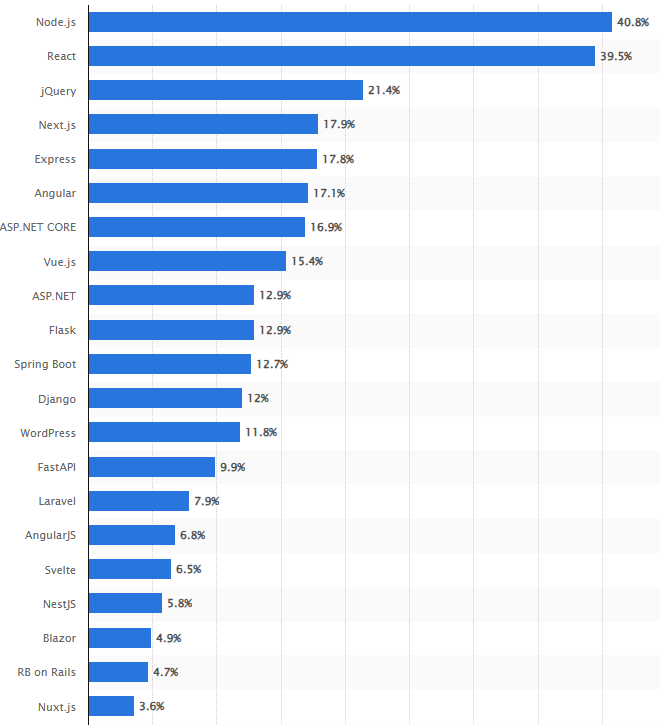
\includegraphics[width=\textwidth]{images/web-frameworks.png}
    \caption{Meistgenutzte Web-Frameworks weltweit (Quelle:\parencite{statista2024})}
    \label{fig:frameworks}
\end{figure}

Bei der Auswahl eines passenden Frameworks fehlt jedoch ein ausgiebiger Vergleich hinsichtlich verschiedener Metriken. Im folgenden Kapitel wird dargestellt, warum ein solcher neuer, umfassender Vergleich notwendig ist.

\section{Aktuelle Situation in der Webentwicklung}

Webanwendungen haben in der heutigen Zeit eine zentrale Rolle im Alltag eingenommen und beeinflussen nahezu jeden Lebensbereich, von Ticket- und Essensbestellungen bis hin zum Online-Shopping (vgl. \autocite[S. 298]{spa-frameworks-2024}). Die Wahl einer passenden Frontendlösung ist hierbei wichtig. 
Die Webentwicklung zeigt hierbei einen klaren Trend in Richtung komponentenbasierter Ansätze für die Frontend-Entwicklung mithilfe von Frameworks wie Angular, React und Vue(vgl. \parencite[S. 43]{js-framework-comparison}). Laut der "State of JavaScript"-Umfrage von 2024 gehören weiterhin Angular,React und Vue zu den drei meist genutzten Frontendframeworks. React bleibt hierbei die Nummer eins hinsichtlich der Nutzung mit 82 Prozent, es folgen Vue.js mit 51 Prozent und Angular mit 50 Prozent. Ebenfalls zu beobachten ist der konstante Anstieg von Svelte mit mittlerweile 26 Prozent (vgl. \parencite {stateofjs2024}).

Die genannten Frameworks legen ihren Fokus auf wiederverwendbare Komponenten, um die Modularität, Wartbarkeit und Skalierbarkeit der Anwendungen zu steigern. (vgl. \autocite [S. 302,303]{spa-frameworks-2024}). 

Alle Frameworks haben ihre Vor- und Nachteile, zeichnen sich aber oft durch einen gewissen Overhead und die eingebaute Komplexität aus. Angular bietet hierbei eine große Skalierbarkeit, während React für komplexe User Interface Elemente sinnvoll ist und Vue.js sich durch die Einfachheit für kleinere Anwendungen auszeichnet (vgl. \parencite[S. 1070]{frontend_frameworks_comparison}). 

Der Entwicklungsaufwand sowie die Wartbarkeit von komponentenbasierten Frameworks kann mit steigender Anwendungsgröße immer komplexer werden. Bei nicht ausreichender Architekturplanung kann eine große technische Schuld entstehen, wie durch die tief verschachtelten Komponentenbäume in React, welche eine Wartbarkeit stark erschweren können (vgl. \parencite[S. 28,29]{comparison-frameworks-scalable-apps}).

Die Performance der Frameworks variiert hinsichtlich ihres Ansatzes, wodurch React und Vue durch die Nutzung eines Virtual DOMs wesentlich schneller bei der Aktualisierung von Elementen sind als Angular und Svelte (vgl. \parencite[S. 61]{js-framework-comparison}).

Trotz einer verbreiteten Nutzung der Frameworks gibt es keinen umfassenden Vergleich zwischen diesen Frameworks. Diese Defizite werden im folgenden Abschnitt genauer aufgezeigt. 

\section{Forschungsstand und bestehende Vergleiche}
\subsection{Vorhande Vergleichsstudien}
Der aktuelle Forschungsstand bringt einzelne Vergleiche, welche aber nur auf Teilaspekte eingehen. Anbei folgt eine Sammlung der bereits vorhandenen Ergebnisse: 
\begin{itemize}
\item \textbf{Performance-Vergleich}: 
Ein wesentlicher Faktor für die Performance von modernen Webanwendungen ist der Umgang mit dem Document Object Model (DOM), da dieser direkten Einfluss auf die Geschwindigkeit von Benutzerinteraktionen hat. 
Frameworks wie React und Vue mit dem Virtual DOM zeigen einen Vorteil durch schnellere Updates, haben aber einen erhöhten Speicherverbrauch. Der Abgleich zwischen Virtual DOM und realem DOM wird dabei als \texttt{Reconciliation} bezeichnet. Angular nutzt die Incremental DOM, welche langsamer, aber dadurch strukturierter für große Anwendungen ist. Das liegt daran, dass Angular Änderungen direkt am tatsächlichen DOM durchführt und dabei auf eine strukturierte Aktualisierung setzt. Svelte besitzt keinen Virtual DOM, wodurch kompakte Builds mit weniger Flexibilität erstellt werden können\parencite[S.61]{js-framework-comparison}
Dies erreicht Svelte, indem es DOM-Manipulationen bereits während der Kompilierungszeit durchführt und dadurch der Browser deutlich weniger Rechenleistung benötigt, was wiederum zu kleineren und schnelleren Bundles führt \parencite[S.26]{comparison-frameworks-scalable-apps}. Durch einen direkten DOM-Zugriff, sind Svelte und Angular schneller als React und Vue.js bei kleineren DOM-Manipulationen. Bei größeren DOM-Operationen sind hingegen React und Vue effizienter. Diese profitieren von ihrem Virtual DOM, da sie viele Operationen bündeln und effizienter abarbeiten können (vgl. \autocite[S.60-62]{js-framework-comparison}). 
Neben der Laufzeitperformance ist auch die Kompilierungszeit bei der Entwicklung relevant. Hierbei zeigt sich, dass Svelte die kürzeste  Kompilierungszeit mit ca. 1,61 Sekunden aufweist. Vue und React sind ebenfalls recht schnell mit einer Kompilierungszeit von ca. 3,96 und 3,07 Sekunden. Angular folgt ein wenig langsamer mit ca. 8,70 Sekunden Kompilierungszeit (vgl. \autocite[S.65]{js-framework-comparison}).
    
\item \textbf{Skalierbarkeit und Wartbarkeit}: Angular bietet standmäßig viele eingebaute Lösungen für Routing, Zustandsverwaltung und Dependency Injection. Ebenfalls fördert Angular die Entwicklung wiederverwendbarer, modularer Komponenten, wodurch mithilfe von TypeScript eine zusätzliche Struktur entsteht. Dies ermöglicht es großen Teams, skalierbare Anwendungen mit ausführlichen Interfaces und Services zu erstellen, da die standardisierte Strukturierung in Angular hierfür besonders geeignet ist. Mit zunehmender Größe der Anwendung wird die Wartbarkeit jedoch immer schwieriger und diese Einhaltung der Strukturen kann die Entwicklungsflexibilität einschränken.
Frameworks wie React bieten eine Modularität welche eine horizontale Skalierung durch die klare Trennung in kleine, unabhängige Komponenten erlaubt und die Wartbarkeit und Erweiterbarkeit begünstigt. Die hohe Flexibilität bedeutet aber gleichzeitig das React auf externe Libraries angewiesen ist wodurch uneinheitlicher Code enstehen kann.
In Frameworks wie React besteht die Gefahr, dass der Komponentenbaum zu tief verschachtelt wird, wodurch die Verfolgung der Datenübertragung immer schwerer wird. 
Vue.js bietet eine einfache und flexible Struktur, wodurch ähnlich wie bei React inkonsistenter Code entstehen kann, wenn keine strikten Standards festgelegt werden. Vue.js nimmt dabei eine Mittelstellung zwischen der Flexibilität von React und dem Funktionsumfang von Angular ein und ermöglicht eine einfache inkrementelle Integration von einzelnen Features
\parencite[S. 25-30]{comparison-frameworks-scalable-apps}.

\item \textbf{Modularität und Wiederverwendbarkeit}: 
Angular fördert die Entwicklung von modularen, wiederverwendbaren Komponenten. Diese sind mithilfe von Typescript klar definiert und erleichtern die Strukturierung großer Anwendungen. 
React bietet ebenfalls eine modulare Struktur, durch welche Komponenten über die ganze Anwendung hinweg wiederverwendbar sind. Durch eine horizontale Skalierung können komplexe React UI in kleine, einfache Komponenten aufgeteilt werden. 
Vue.js Komponenten sind klein, eigenständig und wiederverwendbar aufgebaut und können zum Zusammenbau größerer komplexerer Module verwendet werden. 
Svelte besitzt reaktive Komponenten, die leicht zu erstellen und wiederzuverwenden sind. Hierbei besteht keine Abhängigkeit zu externen Bibliotheken für State-Management aufgrund der kompakten Architektur \cite[S. 24,26] {comparison-frameworks-scalable-apps}.
\end{itemize}

\section{Notwendigkeit eines neuen Vergleichsansatzes}

Die bestehenden Vergleiche fokussieren sich oft nur auf bestimmte Aspekte, wie die Rendering Performance oder Bundle-Größen. Dies sind wichtige Metriken, decken aber nur einen Teilaspekt ab. Hier ist eine ganzheitliche Betrachtung nötig, die auch den Entwicklungsaufwand, die Wartbarkeit sowie Skalierbarkeit berücksichtigt. Bisherige Vergleiche nutzen hauptsächlich Benchmarks und vergleichen anhand dieser die Frameworks. Für eine größere Vergleichsabdeckung ist ein Vergleich der Frameworks bei Nutzung in einem echten Nutzerszenario notwendig. 

\section{Zusammenfassung der Problemstellung}
Der steigende Einsatz von komponentenbasierten Frameworks wie React, Angular, Vue und weiteren bietet viele Vorteile hinsichtlich Wiederverwendbarkeit und Modularisierung. Jedoch entstehen auch Herausforderungen hinsichtlich des Entwicklungsaufwands, der Code-Komplexität und der langfristigen Wartbarkeit.

Die Problemstellung der vorliegenden Forschungsarbeit ergibt sich aus einer Lücke, die bei bisherigen Vergleichen von komponentenbasierten Frameworks besteht. Diese konzentrieren sich oft nur auf spezifische Metriken wie Ladezeiten und stellen dadurch keinen umfassenden Vergleich dar.

Diese Forschungsarbeit schließt die Lücke, indem sie auf eine ganzheitliche Analyse eingeht, die neben Performance-Metriken auch Skalierbarkeit, Wartbarkeit und den tatsächlichen Entwicklungsaufwand untersucht. Der Vergleich erfolgt anhand einer realen Anwendung, um die Frameworks nicht nur unter theoretischen Aspekten, sondern auch in einem praxisnahen Nutzerszenario zu bewerten.

%---
\chapter{Lösungskonzept}
\label{cha:loesungskonzept}

\section{Zielsetzung des Vergleichs}
Ziel des Vergleichs ist es, unterschiedliche Frontend-Technologien anhand ihrer Modularität, ihres Entwicklungsaufwands, ihrer Skalierbarkeit, ihrer Wartbarkeit und ihres State-Managements zu untersuchen.

Untersucht werden das Framework Angular mit einer klassenbasierten Komponentenarchitektur, React mit einer funktionsbasierten Komponentenarchitektur, Web Components als frameworkfreie Lösung einer Komponentenarchitektur und jQuery als herkömmliche Frontend-Lösung.

Der Vergleich findet anhand einer entwickelten E-Commerce-Plattform statt, da diese eine realistische Umgebung für Business-Logik durch Produktverwaltung, Warenkorb und Checkout bietet. Zudem besteht die Möglichkeit einer modularen Erweiterung durch Filter oder Bewertungen. Ein weiterer wichtiger Vergleichspunkt ist das State-Management, da jede Technologie unterschiedliche Ansätze zur Verwaltung des Anwendungszustands verfolgt, soll auch dies ausführlich untersucht werden.

\section{Methodik}
Der Vergleich der Arbeit erfolgt an mehreren Metriken. Es wird zum einen die Modularität und Wiederverwendbarkeit untersucht. Hierbei wird analysiert, inwieweit Komponenten sich wiederverwenden lassen und wie sich ein Projekt mithilfe dieser modularisieren lässt. Ebenfalls  wird die Performance erforscht, wobei alle Performance-Daten, die in den Entwicklungstools des Microsoft Edge-Browsers ermittelt werden können, analysiert werden. Hierzu zählen Ladezeit (Loading Time), Time to First Byte (TTFB), First Contentful Paint (FCP), Largest Contentful Paint (LCP), Time to Interactive (TTI), Renderzeiten der Komponenten, die Anzahl und Größe der Netzwerk-Requests, die JavaScript-Execution-Time sowie die Speichernutzung (Memory Usage). Mithilfe dieser Metriken wird eine umfassende Analyse der Frontend-Frameworks hinsichtlich der Performance ermöglicht. Außerdem wird der Entwicklungsaufwand untersucht. Hierbei wird die Implementationszeit der verschiedenen Features in jedem Framework miteinander verglichen. Ebenfalls wird auf Basis eines gleichen Endprodukts die Code-Komplexität und Lesbarkeit des Codes, der hierfür nötig war, miteinander verglichen. Des Weiteren wird die Skalierbarkeit untersucht, wobei ermittelt werden soll, wie einfach sich weitere Features wie Bewertungen oder Filter in die Anwendung integrieren lassen. Hierbei wird auch in Betracht gezogen, inwieweit bei großen Datenmengen die Performance bestehen bleibt. Ebenfalls untersucht wird die Wartbarkeit. Hierbei wird ermittelt, ob und wie einfach sich Komponenten ändern bzw. erweitern lassen.  

\section{Implementierungsstrategie und Testumgebung}

Die Anwendung besteht aus den Basisfunktionen Produktliste, Warenkorb, Checkout sowie User-Management. Mögliche Erweiterungen sind ein Bewertungssystem der Produkte sowie ein Filter und Suchsystem, um dem User zu ermöglichen, spezifische Produkte zu finden. 
Um einen fairen Vergleich zu ermöglichen, in dem alle Frameworks unter den gleichen Bedingungen verglichen werden, wird die Analyse auf das Frontend fokussiert. Alle Datenbankabfragen verlaufen über ein zentrales Backend, welches die API-Abfragen bearbeitet. 
Außerdem wird sichergestellt, dass die UI-Struktur aller Anwendungen gleich ist. 
Für eine objektive Bewertung der Frameworks wird mithilfe von den Entwicklungstools des Browsers eine Performance Analyse aller entwickelten Lösungen durchgeführt. Hierbei können Messungen wie Ladezeiten und Rendering-Metriken gesammelt und verglichen werden. 

\section{Erwartete Ergebnisse und Nutzen der Analyse}

Das erwartete Ergebnis dieser Arbeit ist es, auf Grundlage der gesammelten Metriken eine fundierte Analyse der untersuchten Frameworks durchzuführen und dabei zu erarbeiten, welches Framework die beste Balance zwischen Performance, Modularität und Entwicklungsaufwand bietet.
Zusätzlich soll untersucht werden, wie sich die Frameworks hinsichtlich Skalierbarkeit und Wartbarkeit unterscheiden und welche hierbei am besten abschneiden.
Die Ergebnisse sollen eine klare Entscheidungshilfe bieten, die dazu dient, für zukünftige Projekte eine fundierte Wahl des passenden Frameworks zu treffen.

%---
\chapter{Implementierung}
\label{cha:implementierung}

Im folgenden Kapitel wird das Lösungskonzept umgesetzt in den 4 ausgesuchten Frontendlösungen. Zusätzlich wird ein zentrales Backend implementiert welches eine Grundlage für den im darauffolgenden Kapitel Vergleich bieten soll. Zunächst wird dargestellt wie die Architektur der gesamten Lösung aufgebaut ist und wie ein allgemeiner Ablauf in den jeweiligen Lösungen aussehen könnte. 

\section{Überblick über die Architektur}
\label{sec:architektur}

In diesem Abschnitt wird die allgemeine Architektur der Lösung dargestellt. Die folgenden Diagramme zeigen den Aufbau der gesamten Anwendung sowie die Interaktionen zwischen Frontend und Backend.

\begin{figure}[H]
    \centering
    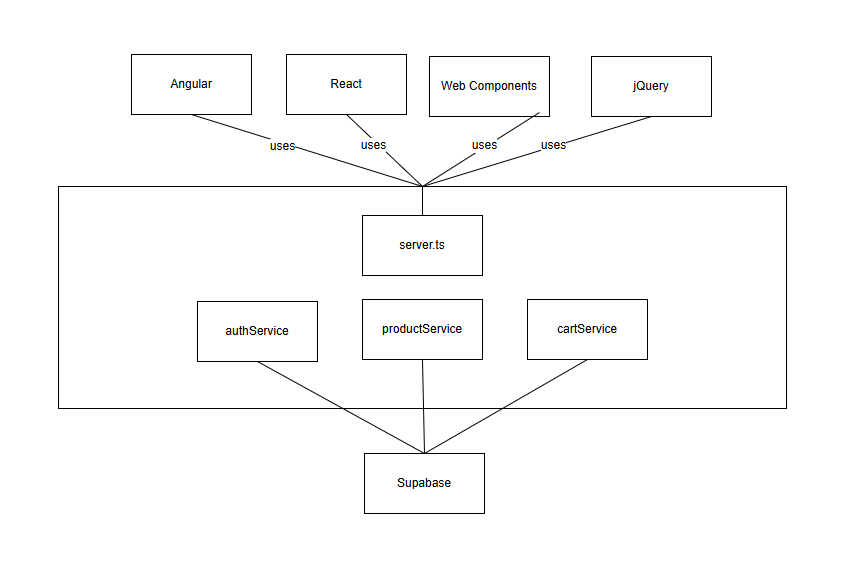
\includegraphics[width=\textwidth]{images/architekturdiagramm}
    \caption{Architekturdiagramm der gesamten Lösung}
    \label{fig:architekturdiagramm}
\end{figure}

Die Architektur besteht aus vier separaten Frontend-Anwendungen (Angular, React, Web Components und jQuery). Diese sind voneinander unabhängig implementiert, kommunizieren aber alle mit dem gleichen zentralen Backend. Das zentrale Backend ist als Node.js Express Server implementiert.

Alle Frontend-Anwendungen greifen hierbei über HTTP-Anfragen auf den Express Server zu. Die Kommunikation erfolgt hierbei über vordefinierte API-Endpunkte, welche in der server.ts definiert sind. Die Anfragen aus dem Server werden in der server.ts empfangen und dann über die passenden Backend-Services weitergeleitet. Die Services lassen sich in die verschiedenen Funktionsbereiche aufteilen: hierbei die Authentifizierung mit dem authService.ts, die Warenkorb-Verwaltung mit dem cartService.ts und die Produktverwaltung mit dem productService.ts. Jeder Service definiert eigene Methoden, welche die vordefinierten Methoden von Supabase nutzen, um auf die Supabase-Datenbank zuzugreifen und mithilfe von CRUD-Operationen Daten zu erstellen, zu lesen, zu aktualisieren oder zu löschen.

\section{Ablaufdiagramm der Anwendungen}
\label{sec:ablauf}

In diesem Abschnitt wird der allgemeine Ablauf der Anwendungen dargestellt. Das folgende Sequenzdiagramm veranschaulicht, wie die verschiedenen Frontendlösungen mit dem zentralen Backend interagieren und welche Schritte bei der Kommunikation zwischen Client und Server ablaufen.

\begin{figure}[H]
    \centering
    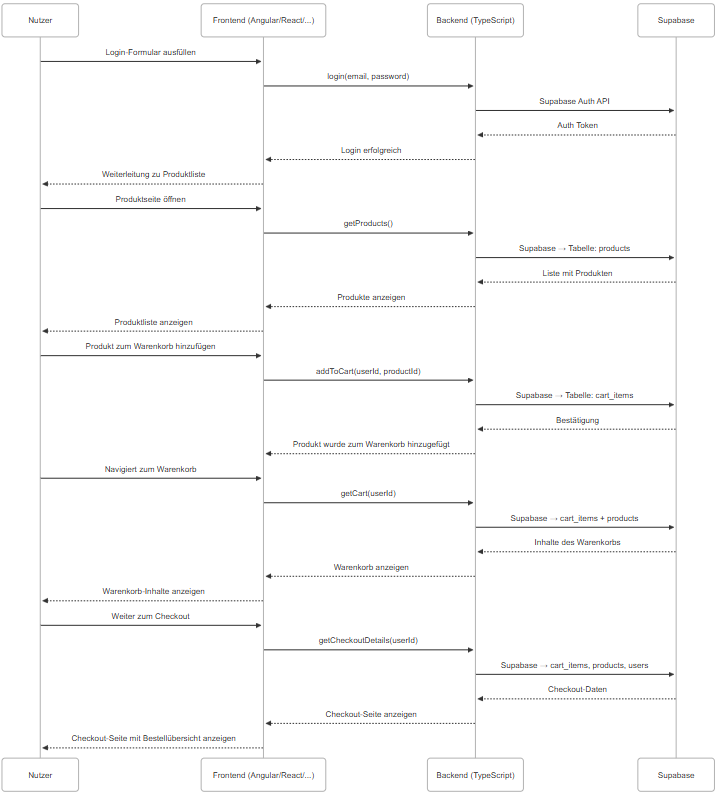
\includegraphics[width=\textwidth]{images/sequenzdiagramm}
    \caption{Überblick über einen beispielhaften Ablauf der Frontendlösungen}
    \label{fig:applikationsstruktur}
\end{figure}

Das Sequenzdiagramm ist 4 Abschnitte aufgeteilt, den Nutzer, dem Frontend, dem Backend und der Supabase Datenbank. Die Kommunikation erfolgt in allen Fällen gleich. 
Zunächst füllt der Nutzer das Login-Formular im Frontend aus und sendet dann per "Login"-Button die Daten an das Backend. Das Backend leitet die Anfrage an Supabase Auth API zur Authentifizierung weiter. Nach einer erfolgreichen Anmeldung wird ein Auth Token zurückgegeben und an das Frontend weitergeleitet. Der Nutzer wird daraufhin bei erfolgreichen Login zu der Produktliste weitergeleitet.

Nun erfolgt das Laden der Produktdaten. Bein öffnen der Seite wird eine Anfrage vom Frontend an das Backend geschickt. Das Backend holt die Produktdaten aus der Tabelle products in Supabase. Die Produkte werden dann zurück an das Frontend übermittelt und angezeigt.

Der Nutzer kann nun die Produktliste ansehen und sich für gewissen Produkte entscheiden. Mit Klick auf den "Zum Warenkorb hinzufügen" Button kann ein Produkt zum Warenkorb hinzugefügt werden. Hierbei wird eine Anfrage vom Frontend an das Backend gesendet mit Angaben zu Benutzer ID- und Produkt-ID. Das Backend speichert die Daten in der Tabelle cart. 

Der Nutzer kann nachdem er alle gewünschten Produkte zum Warenkorb hinzugefügt hat nun zum Warenkorb navigieren. Das Frontend sendet eine Anfrage an das Backend, um die Warenkorbinhalte abzurufen. Das Backend fragt die entsprechenden Daten aus cart und products Tabelle in Supabase ab und sendet den Warenkorbinhalt des Nutzers an das Frontend und zeigt diesen dann an. 

Zuletzt kann der Nutzer wenn er sich vergewissert hat, dass alle gewünschten Produkte im Warenkorb liegen zum Checkout navigieren. Hierbei wird eine Abfrage der Checkout-Daten vom Frontend an das Backend gesendet. Das Backend holt die Daten aus cart und products Tabelle in Supabase. Die Daten werden an das Frontend übermittelt und dem Nutzer als Bestellübersicht dargestellt.

Dieser Ablauf kann in allen Frontendvarianten identisch umgesetzt werden. 


\section{Zentrales Backend-Modul (TypeScript mit Supabase)}
\subsection{Modulstruktur}

Das zentrale Backend besteht aus fünf modular aufgebauten TypeScript-Dateien, die jeweils abgegrenzte Aufgaben übernehmen. Die Verbindung zur Datenbank wird zentral mit Hilfe der \texttt{supabase.ts} initialisiert. Auf dieser Basis stellt die \texttt{server.ts} API-Endpunkte bereit, mithilfe welcher die verschiedenen Frontend-Applikationen ihre Anfragen durchführen können. Hierfür werden verschiedene Services genutzt, die alle kontextabhängige Anfragen an Supabase schicken.

Der erste dieser Services ist der \texttt{authService.ts}. Dieser behandelt alle relevanten Datenbankabfragen hinsichtlich der Authentifizierung des Users. Hierzu gehören Funktionen zur Registrierung, zum Login sowie zur Session-Verwaltung. Ein weiterer Service ist der \texttt{productService.ts}, welcher alle relevanten Datenbankabfragen hinsichtlich der Verwaltung der Produktliste enthält. Dazu gehören Funktionen wie das Fetchen aller Produkte sowie das Fetchen von Produkten anhand einer ID.

Als Nächstes folgt der \texttt{cartService.ts}, welcher sich um alle im Warenkorb relevanten Operationen kümmert. Hierzu gehört das Hinzufügen von Produkten in den Warenkorb und das Abfragen aller im Warenkorb liegenden Produkte.

Es folgt eine klar getrennte Struktur, die durch die \texttt{supabase.ts} als Infrastruktur, der Logik in den jeweiligen Services und den API-Zugriff über die \texttt{server.ts} definiert wird. Alle Services arbeiten über den zentral exportierten Supabase-Client. Durch diese Struktur kann gewährleistet werden, dass alle Frontends ihre Datenbankabfragen über das gleiche Backend durchführen.

\subsection{Supabase-Integration \texttt{supabase.ts}}

Die \texttt{supabase.ts} ist die Schnittstelle zur Supabase-Datenbank. In ihr wird der Supabase-Client initialisiert, mithilfe der Projekt-URL \texttt{SUPABASE\_URL} sowie des API-Keys \texttt{SUPABASE\_ANON\_KEY}. Die entsprechenden Werte werden über eine \texttt{.env}-Datei übermittelt, um keine geheimen Datenbankinformationen über das GitHub-Repository zu verbreiten. Der zentral initialisierte Client kann im Anschluss in allen Services wiederverwendet werden, um Anfragen an Supabase zu schicken.

\subsection{API-Schicht – \texttt{server.ts}}

Die Datei \texttt{server.ts} dient als Verbindung zwischen dem zentralen Backend mit den jeweiligen Services und dem Frontend. In ihr wird ein Express.js-Server definiert, welche HTTP-Endpunkte für die Services wie Authentifizierung, Produkte und Warenkorb definiert.

Webbrowser blockieren standardmäßig Anfragen an einen Server, wenn dieser von einer anderen Domain stammt als die eigene. Wenn das Frontend lokal unter \texttt{localhost:4200} entwickelt wird, das Backend jedoch unter \texttt{localhost:3000} läuft, spricht man von sogenannten Cross-Origin-Anfragen.
Mithilfe von \texttt{cors()} werden Cross-Origin-Anfragen ermöglicht, welche von einer anderen Domain stammen als der Server. Dadurch wird die Kommunikation zwischen Frontend und Backend trotz unterschiedlicher Ursprünge ermöglicht.
Durch \texttt{express.json()} können eingehende JSON-Daten im Request-Body verarbeitet werden.

Ein Beispiel für den Ablauf dieser API-Anfragen ist der \texttt{POST}–Endpoint \texttt{/api/login}, der Benutzer-Login-Anfragen entgegennimmt. Dieser verarbeitet die Login Anfrage mithilfe der Login Funktion aus dem \texttt{authService} und gibt dieses Ergebnis als JSON zurück. 


\begin{lstlisting}[language=TypeScript, caption={Auszug aus \texttt{server.ts}}]
import express from 'express';
import cors from 'cors';
import { login } from './authService';

const app = express();
app.use(cors());
app.use(express.json());

app.post('/api/login', async (req, res) => {
  const { email, password } = req.body;
  const data = await login(email, password);
  res.json(data);
});
\end{lstlisting}

Diese modulare Struktur ermöglicht einfache Erweiterungen bei Integration von weiteren Endpunkten. 

\subsection{Authentifizierungsservice – \texttt{authService.ts}}

Der \texttt{authService.ts} enthält alle Funktionen, die zur Benutzerauthentifizierung benötigt werden. Hierzu gehören die Registrierung und der Login. Bei der Registrierung wird mithilfe des Authentication-Providers Supabase ein neuer Benutzeraccount erstellt, welcher später für alle relevanten Funktionen genutzt werden kann. Darunter fallen z.\,B.\ die Darstellung des nutzerspezifischen Warenkorbs oder das hinzufügen von Produkten in den nutzerspezifischen Warenkorb. Beim Login werden die übergebenen Login-Daten mit der Datenbank verglichen, und es wird zurückgegeben, ob eine erfolgreiche Anmeldung erfolgt ist.
Alle Funktionen werden mithilfe des im \texttt{supabase.ts} definierten Clients durchgeführt.

Ein Beispiel für eine Anfrage an Supabase ist die folgende Login-Funktion aus der \texttt{authService.ts}:

\begin{lstlisting}[language=TypeScript, caption={Login-Funktion im \texttt{authService.ts}}]
import { supabase } from './supabase';

export async function login(email, password) {
  const { data, error } = await supabase.auth.signInWithPassword({
    email,
    password,
  });

  if (error) throw error;  return data;
}
\end{lstlisting}

Diese Struktur ermöglicht eine einfache Erweiterung der in Supabase bestehenden Login-Möglichkeiten, wie z.\,B.\ die Integration von OAuth-Anbietern (z.\,B.\ Google oder GitHub) oder die Implementierung einer Passwort-Zurücksetzen-Funktionalität.

\section{Angular-Implementierung}
\subsection{Struktur und Setup}

Bei der Implementierung wird mit Angular Version 19 gearbeitet. Der Einstiegspunkt in der App findet in der \texttt{main.ts} statt, in welcher mit der \texttt{bootstrapApplication()}-Funktion die App gestartet wird. \texttt{app.config.ts} ist die zentrale Konfigurationsdatei, in welcher das Routing, Provider, HTTP etc. konfiguriert werden kann. Eine genaue Definition der Routen erfolgt in der \texttt{app.routes.ts}. Hier werden alle für die Navigation relevanten Komponenten importiert und in einem Array als Routenobjekte gespeichert. So ist beispielsweise der Pfad zur Warenkorbseite (CartPageComponent) in der app.routes.ts über \texttt{path: 'cart'} definiert. So kann global bei einer durchgeführten Navigation auf diese zugegriffen und navigiert werden. Die \texttt{index.html} definiert die Grundstruktur des HTML der Angular-Anwendung und diese im \texttt{<app-root>} Element.

Die Anwendung ist in viele Komponenten unterteilt. Hierzu gehören Komponenten für die Authentifizierung, Warenkorb, Checkout und Produktliste. Die gesamte Kommunikation mit der Supabase-Datenbank erfolgt über die \texttt{supabase.service.ts}, welche passende API-Anfragen an das zentrale Backend schickt.

\subsection{Integration des Backend-Moduls}

Für eine zentrale Kommunikation mit der Supabase-Datenbank enthält die \texttt{supabase.service.ts} alle relevanten Schnittstellen zum zentralen Backend.
Der Service ist mit \texttt{@Injectable({ providedIn: 'root' })} deklariert, wodurch er zentral für das gesamte Projekt verfügbar ist. Der Supabase-Service wird per Dependency Injection über den Konstruktor in die jeweilige Komponente eingebunden. Der \texttt{HttpClient} wird verwendet, um HTTP-Anfragen wie GET oder POST durchzuführen. Für die Benutzerverwaltung und Authentifizierung bestehen die Methoden \texttt{signUp(email, password)}, \texttt{login(email, password)}. In diesen wird der aktuelle Benutzer für benutzerspezifische Funktionen mithilfe des \texttt{BehaviorSubject} gespeichert. Dadurch wird jederzeit ein Zugriff auf den aktuellen User ermöglicht. Der User kann hierbei Produkte aus der Produktliste, die mithilfe von \texttt{fetchProducts()} geladen werden, zu seinem userspezifischen Warenkorb hinzufügen (\texttt{addToCart(userId, productId, quantity)}) und diesen mit \texttt{getCart(userId)} darstellen.

\subsection{Authentifizierung \texttt{auth.component}}

Die Authentifizierung eines Users erfolgt in der \texttt{auth.component} Komponente. Hier wird mithilfe von Reactive Forms ein Formular erstellt, welches die Nutzerdaten entgegennimmt und bei Absendung abhängig vom Authentifizierungsmodus eine Anmeldung oder Registrierung aus dem Service auslöst. Bei einer erfolgreichen Anmeldung wird der Nutzer auf die Produktlisten-Seite weitergeleitet und kann nun zwischen den verschiedenen Ansichten navigieren. Der Moduswechsel erfolgt durch eine einfache Umschaltfunktion (toggleRegisterMode()), die den State \texttt{isRegistering} entsprechend wechselt.

\subsection{Produktliste \texttt{product-list.component}}

Beim Laden der Seite wird im Angular-\texttt{ngOnInit}-Lifecycle die Methode \texttt{fetchProducts()} aus dem \texttt{SupabaseService} aufgerufen und die Produkte werden in einem Produkt-Array gespeichert.

Im Template wird daraufhin mithilfe der Angular-\texttt{*ngFor}-Direktive die Anzeige in Form einer Liste generiert, die den Namen des Produkts, die Beschreibung, den Preis sowie jeweils einen Button enthält, um das Produkt zum Warenkorb hinzuzufügen.
Durch Klicken des "Add to Cart"-Buttons wird das aktuelle Produkt ausgelesen und die Produkt-ID gemeinsam mit der passenden User-ID über eine Funktion übergeben, wodurch der Artikel dem Warenkorb hinzugefügt wird.
Wenn die Produkte noch nicht geladen sind, wird mithilfe von Angulars \texttt{*ngIf}-Direktive und einem \texttt{<ng-template>} der Text \texttt{"Loading Products..."} angezeigt.


\subsection{Warenkorb \texttt{cart.component}}

Der Warenkorb stellt die vom User hinzugefügten Produkte dar. Beim Aufruf der Warenkorb-Seite wird beim Laden im \texttt{ngOnInit()}-Lifecycle direkt die Methode \texttt{getCartItems()} aufgerufen und speichert die vom Nutzer hinzugefügten Artikel in einem \texttt{cartItems}-Array. Im Template wird jedes Produkt mit dem Produktnamen, Preis und der gekauften Menge dargestellt. Bei einem leeren Warenkorb wird mit \texttt{"your cart is empty"} darauf hingewiesen, dass sich keine Produkte im Warenkorb befinden.

\subsection{Warenkorb-Seite \texttt{cart-page.component}}

Die Warenkorb-Seite verwendet die \texttt{cart.component} als Komponente vollständig wieder und bindet diese neben der passenden Navigation auf den anderen Seiten ein. Wie in allen anderen Komponenten kann mit Hilfe von Angular-Routern durch zwei Buttons eine Navigation auf die anderen Seiten durchgeführt werden.

\lstinputlisting {code/cart-page.component.ts}

Hier ist zu sehen, wie eine einfache Navigation zu beliebigen Angular-Komponenten umsetzbar ist. Die Einbindung einer Komponente erfolgt über den zugehörigen Selector, wie beispielsweise \texttt{<app-cart>}, und ermöglicht dadurch deren Wiederverwendung im Template.

\subsection{Checkout \texttt{checkout.component}}

Die Checkout-Komponente stellt den finalen Überblick über alle im Warenkorb enthaltenen Produkte sowie die Zahlungsinformationen für den Code dar. Hierbei wird die Cart-Komponente wiederverwendet und über das Template mit \texttt{<app-cart>} eingebunden.
Beim Laden der Seite wird im \texttt{ngOnInit}-Lifecycle der Cart die entsprechenden Daten abgerufen und der Gesamtpreis der im Warenkorb enthaltenen Produkte berechnet. Die Zahlungsinformationen sind, genauso wie der "Proceed to Payment"-Button, um den letzten Bestellungsschritt zu simulieren, lesegeschützt. Auch werden zwei Navigationsbuttons, für eine Navigation zu den anderen beiden Seiten dargestellt. Dies wird analog zu den anderen Komponenten implementiert.

\section{React-Implementierung}
\subsection{Struktur und Setup}

Bei der Implementierung wird mit React Version 19 gearbeitet. Der Einstiegspunkt erfolgt über die Datei App.js. Hier wird das Routing mithilfe von BrowserRouter des React-Router Pakets in die Anwendung eingebunden. Dabei werden Routes definiert, die wiederum Route-Elemente zu den verschiedenen Ansichten der Anwendung enthalten. Die Navigation innerhalb der verschiedenen Komponenten erfolgt über Buttons, die mit useNavigate auf andere Komponenten weiterleiten. Im Ordner pages befinden sich alle Hauptkomponenten, darunter die Authentifizierung, die Produktliste, der Warenkorb und der Checkout. Für nutzerspezifische Anfragen wird die Benutzer-ID im localStorage gespeichert und über die Datei authUtils.js verfügbar gemacht. Die Kommunikation mit dem zentralen Backend erfolgt über fetch()-Aufrufe, die passende Endpunkte des Backends ansprechen.

\subsection{Integration des Backend-Moduls}

Die React-Komponenten kommunizieren mit dem zentralen Backend über HTTP-Requests. Hierfür wird \texttt{fetch()} verwendet – etwa für Anfragen wie Login-, Produkt-, Warenkorb- und Checkoutabfragen. Die Daten werden über ein konsistentes Schema im \texttt{JSON}-Format gesendet und empfangen.
Dabei wird ein Backend-Endpunkt angesprochen, der einem festen Schema folgt, beispielsweise \texttt{POST /api/login} oder \texttt{GET /api/products}. Die Benutzer-ID wird – abhängig vom jeweiligen Endpunkt – entweder als URL-Parameter oder im \texttt{Request Body} übermittelt.
Insgesamt ist die Backend-Kommunikation direkt in den jeweiligen Komponenten eingebunden.

\subsection{Authentifizierung \texttt{AuthPage.js}} 

Die Komponente \texttt{AuthPage.js} übernimmt sowohl die Registrierung als auch die Anmeldung eines Benutzers.
Für die Speicherung von Daten wie \texttt{email}, \texttt{password} und dem aktuellen Authentifizierungsmodus wird \texttt{useState} verwendet. Abhängig vom aktuellen Authentifizierungsmodus, der im \texttt{isRegistering}-State gespeichert ist, wird der passende Endpunkt \texttt{/api/signup} oder \texttt{/api/login} verwendet.
Anfragen werden über \texttt{fetch()} als \texttt{POST}-Request im \texttt{JSON}-Format versendet.
Nach einer erfolgreichen Authentifizierung wird die erhaltene \texttt{userId} im \texttt{localStorage} gespeichert, damit sie für spätere nutzerspezifische Funktionen verwendet werden kann. Nach erfolgreicher Anmeldung folgt eine automatische Weiterleitung mithilfe von \texttt{useNavigate('/products')} auf die Produktseite.
Die Login-Komponente stellt ein einfaches Formular mit zwei Eingabefeldern und einem Button dar. Zusätzlich besteht eine Umschaltfunktion (\texttt{toggleRegisterMode()}) in Form eines Buttons, um zwischen Login und Registrierung wechseln zu können.

\subsection{Produktliste \texttt{ProductList.js}} 

Die Komponente \texttt{ProductList.js} stellt eine Liste aller verfügbaren Produkte dar. Beim Laden der Komponente wird im \texttt{useEffect}-Hook ein \texttt{fetch()}-Aufruf an den Endpunkt \texttt{/api/products} durchgeführt. Hierbei werden alle empfangenen Produktdaten im \texttt{products}-State mithilfe von \texttt{useState} gespeichert. Während dieser Datenbankanfrage wird in der Komponente zwischenzeitlich der Text \texttt{"Loading product..."} angezeigt. Sobald die Produkte erfolgreich geladen wurden, werden sie in Form einer Liste dargestellt.

Jeder Eintrag eines Produkts enthält den Namen, die Beschreibung und den jeweiligen Preis des Produkts. Zusätzlich wird für jedes Produkt ein \texttt{Add to Cart}-Button dargestellt, der es ermöglicht, Produkte in den Warenkorb zu legen. Beim Klick auf den "Add to Cart"-Button wird ein \texttt{POST}-Request an \texttt{/api/cart/add} mit den Parametern \texttt{userId}, \texttt{productId} und \texttt{quantity = 1} gesendet. Die \texttt{userId} wird dabei über \texttt{getUserId()} aus der Datei \texttt{authUtils.js} gelesen.

Um das hinzugefügte Produkt im Warenkorb einzusehen, kann mithilfe von zwei Navigationsbuttons entweder zum Warenkorb oder direkt zum Checkout navigiert werden. Dies erfolgt über \texttt{useNavigate}, welches Teil von React Router ist, einem weit verbreiteten Routing-Package für React-Anwendungen. React selbst bietet keine native Routing-Lösung, weshalb \texttt{react-router-dom} hier verwendet wird.

\subsection{Warenkorb-Komponente \texttt{CartComponent.js}} 

Die Komponente \texttt{CartComponent.js} ist für die Darstellung der im Warenkorb enthaltenen Produkte zuständig. Sobald die Komponente geladen wird, erfolgt über den \texttt{useEffect}-Hook ein \texttt{fetch()}-Aufruf an den Endpunkt \texttt{/api/cart?userId=...}. Dadurch werden die Produkte aus dem Warenkorb geladen, die der Nutzer zuvor hinzugefügt hat.

Die \texttt{userId} wird über die Methode \texttt{getUserId()} aus der Datei \texttt{authUtils.js} abgerufen. Für die Anzeige der Produktdetails wird für jedes Produkt ein weiterer \texttt{fetch()}-Aufruf an den Endpunkt \texttt{/api/products/:id} durchgeführt, welcher den Namen,Preis und Stückzahl zu einem Produkt zurückgibt und darstellt.

\subsection{Warenkorb-Seite \texttt{Cart.js}} 

Die Datei \texttt{Cart.js} stellt die komplette Warenkorb-Seite dar.
Sie nutzt die Komponente \texttt{CartComponent.js}, um die Inhalte des Warenkorbs darzustellen. Zusätzlich enthält sie zwei Buttons zur Navigation, einer führt zurück zur Produktliste, der andere zum Checkout. Die Navigation wird dabei über \texttt{useNavigate} aus \texttt{react-router-dom} gesteuert.

\subsection{Checkout-Seite \texttt{Checkout.js}}

Die Komponente \texttt{Checkout.js} stellt die Bestellübersicht vor einem Kauf dar.
Die Produkte im Warenkorb werden erneut mithilfe der Komponente \texttt{CartComponent.js} eingebunden. Beim Laden der Seite wird durch den \texttt{useEffect}-Hook der Gesamtpreis aller Produkte im Warenkorb berechnet. Dabei werden alle Preise der Produkte addiert und als Gesamtbetrag unterhalb der Produktliste dargestellt.

Zusätzlich wird ein Formular für die Zahlungsinformationen angezeigt, in dem Platzhalter eingefügt sind. Ein Button mit der Beschriftung \texttt{"Proceed to Payment"} soll symbolisch auf den möglichen Abschluss des Kaufs hinweisen.
Zur Rücknavigation sind ebenfalls zwei Buttons enthalten, die zurück zur Produktliste bzw. zum Warenkorb navigieren.

\section{Web Components-Implementierung}

\subsection{Struktur und Setup}

Gearbeitet wird mit nativem HTML, CSS und JavaScript. Hierzu werden Custom Elements und das Shadow DOM verwendet. Der zentrale Einstiegspunkt erfolgt über die \texttt{main.js}, welche auch die Routing-Logik für die Anwendung enthält. Der aktuelle Pfad wird mithilfe von \texttt{window.location.pathname} ausgelesen. Mithilfe von \texttt{history.pushState()} wird die Navigation ausgeführt. Die Komponenten werden im Anschluss dynamisch in \texttt{<div id="app">} eingefügt. Es bestehen Komponenten für jeweils Authentifizierung, Produktliste, Warenkorb und Checkout. Alle Komponenten sind in einem Verzeichnis gesammelt und nutzen Services, um Backend-Zugriffe zu handhaben.

\subsection{Integration des Backend-Moduls}

Die Kommunikation mit dem zentralen Backend erfolgt über Service Dateien wie auth-service.js, product-service.js, cart-service.js und checkout-service.js. 
Alle Services handhaben die HTTP-Anfragen an das zentrale Backend. Die Kommunikation erfolgt hierbei über fetch() im JSON-Format. 
Bei der Authentifizierung erfolgt die Kommunikation wie folgt: 

\lstinputlisting {code/auth-service.js}

Der Code definiert eine Klasse AuthService, die zur Handhabung des Authentifizierungsprozesses im Backend genutzt wird. Die Kommunikation erfolgt über HTTP-Anfragen, die mit der Funktion fetch() im JSON-Format gesendet werden. Die Basis-URL des Backends wird im Konstruktor definiert. 

Bei der Funktion signUp wird ein POST-Request an die URL /signup des Backends gesendet. E-Mail und Passwort werden als JSON-Daten im Request-Body übermittelt. Die Antwort wird ebenfalls als JSON-Objekt (response.json()) zurückgegeben. 

Der Login funktioniert ähnlich. Ein POST-Request wird an die URL /login mit denselben Daten gesendet. Zusätzlich werden bei der Anmeldung der zurückgegebene Token sowie die Benutzer-ID im sessionStorage bzw. im localStorage gespeichert, da diese für spätere Funktionalitäten wichtig sind.

\subsection{Authentifizierung (\texttt{auth-component.js})}

Diese Komponente stellt das Login- und Registrierungsformular dar. Der Nutzer kann mithilfe eines Buttons zwischen den beiden Formularen wechseln. Die E-Mail und das Passwort werden hierbei über Input-Felder eingegeben. Beim Abschicken des Formulars über den Button wird passend die Funktion \texttt{authService.login()} oder \texttt{authService.signUp()} aufgerufen. Dies geschieht abhängig vom Boolean-Flag \texttt{isRegistering}, welcher entsprechend gesetzt wird, sobald ein Nutzer zwischen den Ansichten für Login oder Registrierung wechseln kann. Bei einer erfolgreichen Anmeldung wird die \texttt{userId} im \texttt{localStorage} gespeichert, um später nutzerspezifische Anfragen durchführen zu können. Daraufhin erfolgt eine Weiterleitung zur Produktlistenseite.

\subsection{Produktliste (\texttt{product-list-component.js})}

Die Produktliste zeigt alle verfügbaren Produkte aus der Datenbank an. Jedes Produkt besitzt hierbei einen \texttt{Titel}, eine \texttt{Beschreibung}, einen \texttt{Preis} sowie einen Button, um das jeweilige Produkt dem Warenkorb hinzuzufügen. 

Beim Laden der Komponente wird \texttt{productService.fetchProducts()} aufgerufen, um alle Produkte aus der Datenbank zu laden.

Der Nutzer kann ein Produkt zu seinem Warenkorb hinzufügen, indem er auf den \texttt{Add To Cart}-Button klickt. Dabei wird die Funktion \texttt{cartService.addToCart(userId, productId, quantity)} ausgeführt.

Die Navigation zum Warenkorb oder zum Checkout erfolgt über zwei Buttons, welche die Funktion \texttt{navigateTo()} aufrufen und dabei \texttt{window.location.href = \`{}/\$\{page\}.html\`} entsprechend setzen.


\subsection{Warenkorb (\texttt{cart-component.js})}

Die \texttt{Cart}-Komponente zeigt alle Produkte an, die der Nutzer in den Warenkorb gelegt hat. Beim Laden der Komponente wird die Methode \texttt{cartService.getCart(userId)} aufgerufen. Die \texttt{userId} wird hierfür über den \texttt{localStorage} geladen. 

Für jedes Produkt im Warenkorb wird zusätzlich \texttt{productService.getProductById(id)} aufgerufen, um die Details der Produkte aus der Datenbank zu laden.

Die Navigation zurück zur Produktliste oder zum Checkout erfolgt über zwei Buttons. Diese führen die Methode \texttt{navigateTo('/products')} bzw. \texttt{navigateTo('/checkout')} aus und navigieren damit zur entsprechenden Seite.


\subsection{Checkout (\texttt{checkout-component.js})}

Die \texttt{Checkout}-Komponente stellt alle im Warenkorb enthaltenen Produkte sowie eine Anzeige der Zahlungsinformationen dar. Der Warenkorb wird hierbei als Komponente wiederverwendet. Insgesamt wird also eine Gesamtübersicht vor dem Kauf dargestellt.

Beim Laden der Komponente wird der Gesamtpreis aller im Warenkorb liegenden Produkte berechnet. Das Ergebnis wird als Gesamtpreis unterhalb der Liste der Produkte dargestellt. 

Die Eingabefelder für die Zahlungsinformationen sind enthalten, jedoch nicht funktional, sondern dienen lediglich als Platzhalter, um einen Kauf zu simulieren. Gleiches gilt für den Button \texttt{"Proceed to Payment"}.

Für die Navigation auf eine vorherige Seite werden ebenfalls zwei Buttons dargestellt. Diese ermöglichen eine Navigation zu den Produkten sowie zum Warenkorb.


\section{jQuery-Implementierung}

\subsection{Struktur und Setup}

Die jQuery-Implementierung besteht aus mehreren \texttt{.html}-Dateien, welche jeweils eine einzelne Seite der Anwendung darstellen. Die Navigation erfolgt dabei klassisch über die Nutzung von \texttt{<a href="...">}-Links.

Die jeweilige Logik der Seiten befindet sich in separaten JavaScript-Dateien, welche über \texttt{<script>} eingebunden werden. jQuery selbst wird über ein CDN (Content Delivery Network) per \texttt{<script src="...">} eingebunden, anstatt lokal heruntergeladen zu werden.

Jede HTML-Seite lädt das für sie passende jQuery-Skript zur Steuerung der jeweiligen Funktionalität. Die Kommunikation mit dem zentralen Backend erfolgt über die jQuery-Methoden \texttt{\$.\allowbreak ajax()}, \texttt{\$.\allowbreak post()} und \texttt{\$.\allowbreak get()}. Dabei werden die Daten im JSON-Format gesendet und empfangen.

Die Nutzerverwaltung erfolgt über eine \texttt{userId}, welche nach erfolgreichem Login lokal im \texttt{localStorage} gespeichert wird. Mithilfe dieser \texttt{userId} können nutzerspezifische Anfragen durchgeführt werden.

Beim initialen Laden der Seite werden die HTML-Inhalte statisch geladen. Anschließend werden dynamische Inhalte, wie z.\,B.\ Produktlisten oder Warenkorbdaten, mithilfe von jQuery abgerufen und ins \texttt{DOM} geschrieben.

\subsection{Integration des Backend-Moduls}

Die Kommunikation mit dem zentralen Backend erfolgt über HTTP-Requests. Hierfür werden die Methoden \verb|$.ajax()|, \verb|$.post()| und \verb|$.get()| verwendet. Dabei werden die jeweiligen Backend-Endpunkte im Format \texttt{/api/...} angesprochen. Die Datenübertragung erfolgt im \texttt{JSON}-Format.

Nach einer erfolgreichen Registrierung wird die vom Backend zurückgegebene \texttt{userId} im \texttt{localStorage} gespeichert. Diese kann anschließend für weitere Backend-Anfragen genutzt und entweder im Request-Body oder als URL-Parameter mitgesendet werden.

\subsection{Authentifizierung}

Für die Authentifizierung existieren zwei \texttt{.html}-Dateien – eine für die Anmeldung und eine für die Registrierung. Beide enthalten ein einfaches HTML-Formular mit Eingabefeldern für \texttt{E-Mail} und \texttt{Passwort}.

Beim Absenden des Formulars wird dieses mithilfe von \texttt{preventDefault()} abgefangen. Dies soll das standardmäßige Neuladen der Seite verhindern und dient dazu, die Formulardaten asynchron verarbeiten zu können. Anschließend werden die eingegebenen Werte ausgelesen und per \verb|$.post()| an das zentrale Backend gesendet. Nach einer erfolgreichen Anmeldung wird die vom Backend zurückgegebene \texttt{userId} im \texttt{localStorage} gespeichert, und der Nutzer wird automatisch auf die Produktseite weitergeleitet.

\subsection{Produktliste}

Die Produktliste stellt alle Produkte in Form einer Liste dar. Das Grundgerüst besteht aus \texttt{<div id="product-list">} in welches die Produkte dynamisch geladen werden. Beim laden der Seite wird initial mit \verb|$.get('/api/products')| eine Anfrage an das Backend geschickt. Die empfangenen Daten werden in das DOM geschrieben. Jedes Produkt zeigt jeweils den Namen, die Beschreibung, den Preis und einen \texttt{Add to Cart}-Button. 
Mithilfe des jeweiligen Buttons kann ein Produkt in den Warenkorb des Nutzers gespeichert werden. Beim Klick auf den Button \texttt{Add to Cart} wird ein \verb|$.post('/api/cart/add')| mit dem Inhalt \texttt{userId} (aus \texttt{localStorage}), \texttt{productId} und \texttt{quantity = 1} an das Backend geschickt und damit das Produkt im Warenkorb des Nutzers gespeichert.
Zur Navigation zum Warenkorb oder zum Checkout stehen 2 Buttons zur Verfügung, welche beide mithilfe von \texttt{<a href="...">}-Links den Nutzer auf die entsprechende Seite navigieren. 

\subsection{Warenkorb-Komponente}

Der Warenkorb stellt alle vom Nutzer hinzugefügten Produkte dar. Hierbei wird beim Laden der Seite direkt der aktuelle Nutzer mithilfe der im \texttt{localStorage} gespeicherten \texttt{userId} ausgelesen. Mit \verb|$.get('/api/cart?userId=...')| wird eine Anfrage an das Backend geschickt, um die nutzerspezifischen Warenkorbdaten zu erhalten.

Für die im Warenkorb enthaltenen Produkte wird nochmals ein \verb|$.get('/api/products/:id')| durchgeführt. Dieser Aufruf dient dazu, die zugehörigen Produktdetails (Name, Preis etc.) zu erhalten. Diese Informationen werden anschließend dynamisch mit \verb|$('#cart').append(...)| in das DOM geschrieben.

Die Navigation zurück zur Produktliste sowie zum Checkout erfolgt über zwei Buttons, welche mit \texttt{<a href="...">}-Links den Nutzer auf die jeweilige Seite weiterleiten.


\subsection{Checkout-Seite}

Der Checkout stellt den finalen Bestellvorgang dar und zeigt hierfür alle im Warenkorb enthaltenen Artikel sowie die Zahlungsinformationen. Beim Aufruf der Seite wird der \texttt{userId} aus dem \texttt{localStorage} ausgelesen. Diese wird verwendet, um mit \verb|$.get('/api/cart?userId=...')| die im Warenkorb enthaltenen Produkte vom zentralen Backend abzurufen. 

Für jedes Element im Warenkorb werden erneut mit \verb|$.get('/api/products/:id')| die Produktinformationen der Produkte geladen. Alle Produkte werden daraufhin im DOM angezeigt. Gleichzeitig wird daraus der Gesamtpreis berechnet, indem \texttt{preis * menge} für jedes Produkt addiert wird. 

Die Zahlungsinformationen sowie der \texttt{"Proceed to Payment"}-Button sind rein symbolisch und führen keine echte Transaktion aus. Zusätzlich befinden sich am unteren Rand der Seite zwei Navigationsbuttons, die zurück zur Produktliste bzw. zum Warenkorb führen.

\section{Zusammenfassung}

Die vier verschiedenen Frameworks wurden implementiert und haben hierfür verschiedene Lösungsansätze genutzt. Alle verwenden das zentrale Backend, mit dem Datenbankoperationen durchgeführt werden können. Hierfür wird die \texttt{server.ts}-Datei genutzt, welche die Endpunkte für die HTTP-Anfragen definiert. Die entsprechenden Services greifen dann über CRUD-Operationen auf die Supabase-Datenbank zu und holen sich hierüber die benötigten Daten. Für den Zugriff auf die Datenbank wurden verschiedene Lösungen umgesetzt. Ebenfalls wurden für State-Management und Routing verschiedene Lösungen passend zum jeweiligen Framework umgesetzt. Jede dieser Lösungen hat gewisse Vor- und Nachteile. Diese müssen nun ausführlich dargestellt und verglichen werden. Für den kommenden Vergleich im Kapitel Evaluierung werden auch weitere Aspekte untersucht, die nun mit der abgeschlossenen Implementierung betrachtet werden können. Hierzu gehören die Performance anhand von Messungen bestimmter Metriken, die Wartbarkeit, die Erweiterbarkeit, Skalierbarkeit, der Entwicklungsaufwand, die Modularität, die Wiederverwendbarkeit und die Komplexität des Codes.


\chapter{Inbetriebnahme}
Dieses Kapitel beschreibt die notwendigen Schritte, um die entwickelte Anwendung lokal zu installieren und auszuführen. Die Inbetriebnahme umfasst sowohl das zentrale Backend als auch die vier verschiedenen Frontend-Anwendungen, die auf Angular, React, Web Components und jQuery basieren.

\section{Voraussetzungen}
Bevor die Anwendung gestartet werden kann, müssen folgende Software-Komponenten installiert sein:
\begin{itemize}
    \item \textbf{Node.js} Version 18.15.0
    \item \textbf{npm} Version 9.5.0 
    \item \textbf{Git} Version 2.33.0
\end{itemize}

\section{Repository klonen}
Das Git-Repository der Anwendung muss zunächst lokal geklont werden. Dies geschieht mit folgendem Befehl:
\begin{verbatim}
git clone https://github.com/Kechter/Bachelorarbeit.git
\end{verbatim}

\section{Installation der Abhängigkeiten}
Nach dem Klonen des Repositories müssen für jede der Anwendungen die Abhängigkeiten installiert werden. 

\subsection{Angular}
Navigiere in das Angular-Verzeichnis und installiere die Abhängigkeiten mit:
\begin{verbatim}
cd angular-app
npm install
\end{verbatim}

\subsection{React}
Navigiere in das React-Verzeichnis und installiere die Abhängigkeiten mit:
\begin{verbatim}
cd react-app
npm install
\end{verbatim}

\subsection{Web Components}
Navigiere in das Web Components-Verzeichnis und installiere die Abhängigkeiten mit:
\begin{verbatim}
cd web-components-app
npm install
\end{verbatim}

\subsection{jQuery}
Navigiere in das jQuery-Verzeichnis und installiere die Abhängigkeiten mit:
\begin{verbatim}
cd jquery-app
npm install
\end{verbatim}

\section{Starten der Anwendungen}
Die Anwendungen können mit den folgenden Befehlen gestartet werden:

\subsection{Angular}
\begin{verbatim}
ng serve
\end{verbatim}
Die Anwendung ist dann unter \texttt{http://localhost:4200} erreichbar.

\subsection{React}
\begin{verbatim}
npm start
\end{verbatim}
Die Anwendung ist dann unter \texttt{http://localhost:3000} erreichbar.

\subsection{Web Components}
\begin{verbatim}
npx serve
\end{verbatim}
Die Anwendung ist dann unter \texttt{http://localhost:3000} erreichbar.

\subsection{jQuery}
\begin{verbatim}
npx serve
\end{verbatim}
Die Anwendung ist dann unter \texttt{http://localhost:3000} erreichbar.

\section{Backend kompilieren und starten}
Das zentrale Backend muss zuerst kompiliert werden, bevor es gestartet werden kann.

\begin{verbatim}
cd shared-backend
npm install
npm run build
node dist/server.js
\end{verbatim}

Das Backend ist nun unter \texttt{http://localhost:3001} erreichbar.

\section{Zusammenfassung}
Nachdem alle Anwendungen und das Backend erfolgreich gestartet wurden, können diese lokal getestet und verwendet werden. Weitere Konfigurationsoptionen werden im Kapitel \textit{Konfiguration} beschrieben.

%---
\chapter{Evaluierung}

Die zuvor gezeigten Implementierungslösungen gilt es nun anhand passender Metriken zu evaluieren. Dabei wurde zuvor eine Auswahl an Kriterien festgelegt, welche relevante Aspekte von modernen Webanwendungen umfassen, um dadurch eine ganzheitliche Bewertung zu ermöglichen. Das Ziel ist es, die verwendeten Frontendtechnologien, Angular, React, Web Components und jQuery systematisch miteinander zu vergleichen. Das zentrale Backend dient als Grundlage für alle Lösungen und kann dadurch bei dem Vergleich außer Acht gelassen werden.

Die Evaluierung erfolgt anhand verschiedener Qualitätsmerkmale einer Webanwendung, darunter die Performance, Wartbarkeit, Erweiterbarkeit, Skalierbarkeit, Entwicklungsaufwand, Modularität und Code-Komplexität. Damit lassen sich neben technischen Unterschieden auch praxisorientierte Rückschlüsse für die Technologiewahl ziehen. 

\section{Performance}
Ziel der Performance Analyse ist es, die Ladezeit sowie weitere Werte zu ermitteln und mithilfe dieser zu bestimmten, wie sich die verschiedenen Implementierungen hinsichtlich ihrer Performance voneinander unterscheiden.
Die Messungen wurden mit den \texttt{Edge Dev Tools} durchgeführt, welche sowohl einen \texttt{Performance}- als auch einen \texttt{Netzwerk}-Tab bereitstellen. In diesem lassen sich sämtliche relevanten Metriken auslesen und begutachten. Im Rahmen der Analyse wurden insbesondere folgende Werte betrachtet:
\begin{itemize}
  \item \texttt{Loading Time}
  \item \texttt{DOMContentLoaded}
  \item \texttt{TTFB} (Time to First Byte)
  \item \texttt{FCP} (First Contentful Paint)
  \item \texttt{LCP} (Largest Contentful Paint)
  \item \texttt{TTI} (Time to Interactive)
  \item Renderzeiten einzelner Komponenten
  \item Anzahl der \texttt{Netzwerk-Requests}
  \item Größe der geladenen Ressourcen
  \item \texttt{JavaScript}-Ausführungszeit
\end{itemize}

Für möglichst realistische und vergleichbare Ergebnisse wird die Messung ohne eine künstliche Netzwerkdrosselung durchgeführt. Für eine aussagekräftige Messung wurde der Cache deaktiviert, wodurch bei jedem Neuladen der Seite (via \texttt{F5}) sämtliche Ressourcen neu vom lokalen Webserver geladen werden. 
Alle Seiten werden mit den gleichen Daten aus einer Datenbank befüllt, wodurch ein fairer Vergleich der Lösungen ermöglicht wird. 
Verglichen werden alle relevanten Seiten der Anwendungen, beginnend mit dem Login, Produktliste, Warenkorb und anschließend dem Checkout.
Beim Laden der Seite werden mehrere Refreshes durchgeführt und ein Wert verwendet, welcher den durchschnittlichen Ladegeschwindigkeiten entspricht.

\section{Vergleich der Messergebnisse}
\subsection{Vergleich der Login-Seite}

\begin{table}[H]
\centering
\caption{Performance-Messung - Login Page}
\begin{tabular}{|p{3.5cm}|p{2.5cm}|p{2.5cm}|p{2.5cm}|p{2.5cm}|}
\hline
\textbf{Metrik}                  & \textbf{React} & \textbf{Angular} & \textbf{Web Components} & \textbf{jQuery} \\ \hline
Loading Time                     & 231 ms        & 278 ms           & 257 ms                 & 135 ms          \\ \hline
DOMContentLoaded                 & 118 ms        & 227 ms           & 91 ms                  & 85 ms           \\ \hline
TTFB                             & 49 ms        & 31 ms            & 4 ms                   & 6 ms            \\ \hline
FCP                              & $\approx$0.489 s & $\approx$0.09 s & $\approx$0.06 s        & $\approx$0.072 s \\ \hline
LCP                              & $\approx$0.489 s & $\approx$0.09 s & $\approx$0.06 s        & $\approx$0.072 s \\ \hline
TTI                              & $\approx$0.515 s & $\approx$0.3 s & $\approx$0.1 s         & $\approx$0.072 s \\ \hline
Renderzeiten der Komponenten     & $\approx$62 ms & $\approx$12 ms   & $\approx$12 ms         & - \\ \hline
Netzwerk-Requests (Anzahl)       & 7              & 24               & 13                    & 6               \\ \hline
Größe der geladenen Dateien      & 340 KB / 1.7 MB & 2.5 MB          & 12.3 KB / 15.8 KB     & 43.6 KB / 118 KB \\ \hline
JS-Execution-Time                & $\approx$61 ms       & $\approx$120 ms          & $\approx$19 ms                 & $\approx$29 ms         \\ \hline
\end{tabular}
\end{table}

Bei der Betrachtung der Messergebnisse, lässt sich sagen, dass die Messwerte bei der Loginseite relativ ähnlich sind, da keine großen Komponenten bzw. Seiten erstellt wurden. Dennoch lassen sich hier bereits deutliche Unterschiede erkennen.

jQuery schneidet insgesamt am besten ab. Die schnellste Ladezeit von 135 ms, die schnellste TTI von 0,072 Sekunden und eine solide JavaScript Execution Time von 29 ms zeigen, dass jQuery bei kleineren Seiten sehr effiziente Ladezeiten aufweist.

Web Components schneiden ähnlich gut ab, allerdings mit einer leicht erhöhten Ladezeit von 257 ms. Dafür ist die TTI mit 0,1 Sekunden deutlich besser als bei React und Angular. Auch die JavaScript Execution Time von 19 ms ist hervorragend und besser als die getesteten Ansätze.

React und Angular erreichen bei der Loginseite insgesamt schlechtere Werte. Die TTI von React (0,515 Sekunden) ist die langsamste, gefolgt von Angular (0,3 Sekunden). Besonders Angular leidet unter einer hohen JavaScript Execution Time von 120 ms und einer großen Dateigröße von 2,5 MB.

Ein Blick auf FCP und LCP zeigt, dass jQuery und Web Components besonders schnell rendern, während React und Angular auch hier wieder langsamer sind. React hat hier mit 0,489 Sekunden die schlechtesten Werte, während Angular mit 0,09 Sekunden solide, aber nicht optimal ist.
\subsection{Vergleich der Produkt-Seite}

\begin{table}[H]
\centering
\caption{Performance-Messung - Produkt Page}
\begin{tabular}{|p{3.5cm}|p{2.5cm}|p{2.5cm}|p{2.5cm}|p{2.5cm}|}
\hline
\textbf{Metrik}                  & \textbf{React} & \textbf{Angular} & \textbf{Web Components} & \textbf{jQuery} \\ \hline
Loading Time                     & 223 ms        & 522 ms           & 295 ms                 & 405 ms          \\ \hline
DOMContentLoaded                 & 115 ms        & 402 ms           & 114 ms                 & 131 ms          \\ \hline
TTFB                             & 45 ms        & 198 ms           & 63 ms                  & 265 ms          \\ \hline
FCP                              & $\approx$0.29 s  & $\approx$0.29 s  & $\approx$0.2 s        & $\approx$0.068 s  \\ \hline
LCP                              & $\approx$0.43 s  & $\approx$0.29 s  & $\approx$0.26 s       & $\approx$0.25 s \\ \hline
TTI                              & $\approx$0.43 s  & $\approx$0.49 s  & $\approx$0.26 s       & $\approx$0.25 s \\ \hline
Renderzeiten der Komponenten     & $\approx$58 ms & $\approx$17 ms   & $\approx$27.8 ms          & -  \\ \hline
Netzwerk-Requests (Anzahl)       & 9              & 25               & 15                    & 5               \\ \hline
Größe der geladenen Dateien      & 343 KB / 1.7 MB & 2.5 MB          & 13.7 KB / 17.4 KB     & 44.7 KB / 118 KB \\ \hline
JS-Execution-Time                & $\approx$58 ms       & $\approx$129 ms          & $\approx$27 ms                & $\approx$29 ms         \\ \hline
\end{tabular}
\end{table}

Beim Laden der Produktliste zeichnen sich ebenfalls Unterschiede zwischen den Technologien ab. jQuery und Web Components schneiden am besten ab. Die TTI ist mit 0,25 Sekunden (jQuery) und 0,26 Sekunden (Web Components) am schnellsten. jQuery zeigt zudem eine sehr schnelle FCP von 0,068 Sekunden und eine solide JavaScript Execution Time von 29 ms. Schwächen von jQuery sind hingegen die lange Ladezeit der gesamten Anwendung beim vollständigen Laden im Browser, in Höhe von 405 ms, sowie der hohe TTFB von 265 ms.

Web Components zeigen ebenfalls gute Werte mit einer TTI von 0,26 Sekunden und einer schnellen JavaScript Execution Time von 27 ms. Die Dateigröße von 13,7 KB / 17,4 KB ist die kleinste im Vergleich, was sich positiv auf die Performance auswirkt. Schwächen sind ein TTFB von 63 ms sowie eine leicht erhöhte LCP von 0,26 Sekunden.

React hat mit 223 ms die schnellste Ladezeit, jedoch sind die TTI von 0,43 Sekunden, die FCP von 0,29 Sekunden und die LCP von 0,43 Sekunden im Vergleich höher. Die JavaScript Execution Time von 58 ms ist ebenfalls schlechter als bei Web Components und jQuery. Auch die Dateigröße von 343 KB / 1,7 MB fällt hier eher negativ auf.

Angular erzielt insgesamt die schwächsten Ergebnisse. Die Ladezeit beträgt 522 ms und die TTI ist mit 0,49 Sekunden die langsamste. Auch die JavaScript Execution Time von 129 ms ist mit Abstand am höchsten. Zudem verursacht Angular mit 25 Netzwerk-Requests die meisten Aufrufe und hat mit 2,5 MB die größte Dateigröße.

\subsection{Vergleich der Warenkorb-Seite}

\begin{table}[H]
\centering
\caption{Performance-Messung - Warenkorb Page}
\begin{tabular}{|p{3.5cm}|p{2.5cm}|p{2.5cm}|p{2.5cm}|p{2.5cm}|}
\hline
\textbf{Metrik}                  & \textbf{React} & \textbf{Angular} & \textbf{Web Components} & \textbf{jQuery} \\ \hline
Loading Time                     & 358 ms        & 482 ms           & 431 ms                 & 715 ms          \\ \hline
DOMContentLoaded                 & 115 ms        & 258 ms           & 118 ms                 & 95 ms           \\ \hline
TTFB                             & 50 ms         & 13 ms            & 122 ms                 & 90 ms           \\ \hline
FCP                              & $\approx$0.125 s & $\approx$0.19 s & $\approx$0.263 ms      & $\approx$0.09 s \\ \hline
LCP                              & $\approx$0.45 s & $\approx$0.19 s & $\approx$0.45 s      & $\approx$0.77 s \\ \hline
TTI                              & $\approx$0.48 s & $\approx$0.35 s & $\approx$0,45 s        & $\approx$0.8 s \\ \hline
Renderzeiten der Komponenten     & $\approx$15 ms      & $\approx$11 ms            & $\approx$20 ms      & -           \\ \hline
Netzwerk-Requests (Anzahl)       & 19            & 35               & 19                     & 18              \\ \hline
Größe der geladenen Dateien      & 347 KB / 1.7 MB & 2.5 MB         & 15.9 KB / 18.4 KB      & 50.7 KB / 122 KB \\ \hline
JS-Execution-Time                & $\approx$71 ms & $\approx$72 ms          & $\approx$20 ms                 & $\approx$33 ms          \\ \hline
\end{tabular}
\end{table}

Beim Laden des Warenkorbs zeichnen sich erste Veränderungen ab. Angular schneidet mit guten Werten ab. Die TTI ist mit 0,35 Sekunden die schnellste. Auch die FCP, LCP und JavaScript Execution Time sind bei Angular am geringsten. Schwächen von Angular sind die größte Dateigröße von 2,5 MB und die vielen Netzwerk-Anfragen.

Web Components zeigt ebenfalls gute Werte mit einer TTI von 0,45 Sekunden sowie einer schnellen JavaScript Execution Time von 20 ms. Web Components hat eine kleine Dateigröße sowie relativ wenige Requests. Hohe Werte hat Web Components jedoch bei der TTFB von 122 ms sowie einer erhöhten LCP.

Direkt darauf folgt React mit der gleichen TTI von 0,48 Sekunden, aber einer langsameren JavaScript Execution Time. React besitzt eine niedrige FCP, dafür aber eine erhöhte LCP. Die Dateigröße ist ähnlich wie bei Angular relativ hoch, ebenso wie die JavaScript Execution Time, die vergleichsweise lang ist.

jQuery hat diesmal die schlechtesten Werte mit einer langen TTI von 0,8 Sekunden sowie einer hohen LCP. Die FCP hingegen ist die geringste mit 0,09 Sekunden, ebenso wie die Anzahl der Netzwerk-Requests und die JavaScript Execution Time von 33 ms.

\subsection{Vergleich der Checkout-Seite}

\begin{table}[H]
\centering
\caption{Performance-Messung - Checkout Page}
\begin{tabular}{|p{3.5cm}|p{2.5cm}|p{2.5cm}|p{2.5cm}|p{2.5cm}|}
\hline
\textbf{Metrik}                  & \textbf{React} & \textbf{Angular} & \textbf{Web Components} & \textbf{jQuery} \\ \hline
Loading Time                     & 1.070 ms      & 450 ms           & 376 ms                 & 850 ms          \\ \hline
DOMContentLoaded                 & 130 ms        & 324 ms           & 121 ms                 & 150 ms          \\ \hline
TTFB                             & 56 ms        & 57 ms            & 60 ms                  & 80 ms            \\ \hline
FCP                              & $\approx$0.2 s & $\approx$0.11 s & $\approx$0.2 s        & $\approx$0.12 s \\ \hline
LCP                              & $\approx$0.2 s & $\approx$0.34 s & $\approx$0.26 s       & $\approx$0.8 s \\ \hline
TTI                              & $\approx$0.45 s & $\approx$0.45 s & $\approx$0.26 s       & $\approx$0.85 s \\ \hline
Renderzeiten der Komponenten     & $\approx$83 ms         & $\approx$18 ms            & $\approx$223 ms                  & - ms           \\ \hline
Netzwerk-Requests (Anzahl)       & 41            & 83               & 31                    & 31              \\ \hline
Größe der geladenen Dateien      & 359 KB / 1.7 MB & 2.5 MB         & 21.8 KB               & 57.4 KB         \\ \hline
JS-Execution-Time                & $\approx$84 ms       & $\approx$53 ms          & $\approx$30 ms               & $\approx$52 ms         \\ \hline
\end{tabular}
\end{table}

Beim Laden der Checkout-Seite zeigen sich erneut deutliche Unterschiede zwischen den Frameworks. Web Components schneiden hier am besten ab. Die TTI ist mit 0,26 Sekunden die niedrigste im Vergleich, ebenso die JavaScript Execution Time mit 30 ms. Auch die Dateigröße von nur 21,8 KB und die moderate Anzahl von 31 Netzwerk-Requests tragen zur guten Gesamtleistung bei. Schwächen finden sich jedoch bei der Renderzeit der Komponenten (223 ms) sowie beim TTFB von 60 ms.

Angular zeigt solide Werte mit einer TTI von 0,45 Sekunden, die im Vergleich mit React identisch ist. Besonders positiv fällt die FCP von 0,11 Sekunden auf. Auch die JavaScript Execution Time von 53 ms ist akzeptabel. Negativ wirkt sich erneut die hohe Dateigröße von 2,5 MB und die sehr hohe Anzahl an Netzwerk-Requests (83) aus.

React hat mit 1.070 ms die längste Ladezeit. Die TTI liegt ebenfalls bei 0,45 Sekunden, jedoch mit der höchsten JavaScript Execution Time (84 ms). Auch die Renderzeit der Komponenten (83 ms) ist deutlich höher als bei Angular. Die Dateigröße von 359 KB / 1,7 MB ist vergleichsweise groß.

jQuery zeigt bei dieser Seite die schwächsten Ergebnisse. Mit einer TTI von 0,85 Sekunden und einer LCP von 0,8 Sekunden ist die Seite deutlich später interaktiv als bei allen anderen Frameworks. Die FCP von 0,12 Sekunden ist zwar solide, jedoch ist auch die Ladezeit mit 850 ms recht hoch. Positiv hervorzuheben sind die vergleichsweise geringe Dateigröße (57,4 KB) und die JavaScript Execution Time von 52 ms.

\subsection{Fazit der Performance-Messungen}

Insgesamt lässt sich beobachten, dass Web Components und jQuery auf wenig komplexen Seiten (Login, Produktseite) die besten Ergebnisse erzielen. Je komplexer die Seiten werden (Warenkorb, Checkout), desto mehr verbessert sich die Performance von Angular, während jQuery zunehmend an Effizienz verliert. Web Components bleibt über alle Seiten hinweg eine konstant gute Lösung und erreicht meist in den Performance-Messungen Platz zwei. React bewegt sich durchgehend im Mittelfeld und landet in den meisten Fällen auf dem dritten Platz.

\section{Wartbarkeit}
Die Wartbarkeit eines Systems lässt bestimmen Anhand wie einfach folgende Dinge getan werden können: 
\begin{itemize}
    \item \textbf{Fehlerbehebung:} Wie leicht können Bugs identifiziert und behoben werden?
    \item \textbf{Anpassungen:} Wie schnell lassen sich bestehende Komponenten anpassen, um neue Anforderungen zu erfüllen?
    \item \textbf{Refactoring:} Wie einfach kann der Code umstrukturiert werden, um die Qualität zu verbessern, ohne die Funktionalität zu verändern?
\end{itemize}

\subsection{Fehlerbehebung}

Angular bietet durch die Nutzung von Typescript bereits zur Compile-Zeit eine grundlegende Typensicherung. Dadurch können z.B. falsche Typen und fehlende Imports frühzeitig erkannt werden. Mithilfe der Angular CLI werden viele Fehler in der Konsole dargestellt und können somit schneller behoben werden. 

React-Code kann mithilfe der Developer Tools auf Fehler analysiert werden. Hierbei können beispielsweise mithilfe eines Browser Plugins die Komponenten und Datenflüsse detailliert dargestellt werden. In React können Error Boundaries implementiert werden, welche bei einem Fehler die Anwendung isoliert darstellen und den Fehler übermitteln. Dies hat den Vorteil, dass nicht die gesamte Anwendung abstürzt, sondern nur der betroffene Komponentenbaum. Dadurch können gezielt Fehlermeldungen angezeigt oder alternative Inhalte gerendert werden. Ebenfalls bietet React eine Typescript Unterstützung, wodurch wie bei Angular falsche Typen zur Compilezeit erkannt und behoben werden können. 

Web Components bietet keine Framework-Unterstüzung für die Fehlerbehebung. Mit Web Components muss die Fehlerbehandlung manuell implementiert werden. 

jQuery bietet ebenfalls keine umfangreiche Fehlerbehebungsunterstützung, ermöglicht jedoch zumindest mit AJAX-Methoden wie .ajax(), .get(), oder .post() ein standardisiertes Error Handling für Serveranfragen.

\subsection{Anpassungen}

Angular bietet eine klare Strukturierung durch Module und Services. Dadurch können gezielte Änderungen vorgenommen werden, um bestimmte Strukturen anzupassen. Die Typisierung durch TypeScript hilft dabei, Fehler frühzeitig zu erkennen. Bei größeren Anpassungen ist die strikte Architektur von Angular hilfreich, da sie eine konsistente Handhabung ermöglicht. Dies kann jedoch aufwändig werden, wenn viele verschachtelte Komponenten betroffen sind.

React bietet Flexibilität durch funktionale Komponenten und Hooks, was Anpassungen prinzipiell unkompliziert macht. Der Virtual DOM erleichtert Änderungen durch eine direkte Visualisierung. Die hohe Flexibilität kann bei größeren Projekten jedoch auch zum Nachteil werden, da eigene sinnvolle Strukturen geschaffen werden müssen, um Fehler bei Anpassungen zu vermeiden.

Web Components bieten ebenfalls eine hohe Flexibilität durch die Unabhängigkeit von einem Framework. Anpassungen sind möglich, indem einzelne Komponenten angepasst oder erweitert werden. Bei komplexen Anwendungen kann die fehlende Strukturierung jedoch zu einem höheren Zeitaufwand führen.

jQuery ermöglicht durch die direkte Manipulation des DOM einfache Anpassungen, die jedoch oft unübersichtlich werden. Änderungen in größeren Projekten sind zwar möglich, aber schwerer nachzuvollziehen, da keine klare Struktur vorgegeben ist.

\subsection{Refactoring}

\section{Erweiterbarkeit}

Die mögliche Erweiterbarkeit der Frontendlösungen wird anhand eines Produktfilters skizziert. Hierbei wird analysiert wie einfach eine solche Erweiterung in den jeweiligen Lösungen möglich wäre. 

\subsection{Angular}

In Angular müsste für die Logik des Filters ein zentraler Filterservice implementiert werden. Dieser Service (\texttt{filterService.ts}) wird in der \texttt{ProductListComponent.ts} importiert und angewandt. Im HTML der Produktliste wird mithilfe eines Filterformulars auf den Service zugegriffen, um die gefilterten Produkte anzuzeigen.

\subsection{React}

In React müsste die Logik des Filters in einer zentralen useFilter.js implementiert werden. Diese kann daraufhin in der ProductListComponent importiert und mithilfe von Hooks verwendet werden. Zusätzlich muss die render Logik passend angepasst werden. 

\subsection{Web Components}

In Web Components müsste die Logik des Filters in einer eigenen produkt-filter.js implementiert werden. Das benutzerdefinierte Element muss daraufhin muss dann in der Produktliste eingefügt werden. 

\subsection{jQuery}

In jQuery könnte die Logik des Filters in einer filterService.js implementiert werden. 
Dieser Service wird in der product.js eingefügt um die Logik zu nutzen und das Filterformular in der \texttt{products.html} hinzufügen. 

\section{Skalierbarkeit}

Skalierbarkeit beschreibt die Fähigkeit eines Systems, bei wachsendem Umfang weiterhin effizient zu funktionieren. Die untersuchten Frameworks unterscheiden sich hier vor allem in der Art und Weise, wie sie Modularisierung, Datenmanagement und Komponentenstruktur unterstützen.

\subsection{Angular}
\todo{neu formulieren}

Angular bietet durch seine modulare Architektur eine gute Skalierbarkeit. Die Verwendung von Modulen (\texttt{app.routes.ts}, \texttt{app.config.ts}) ermöglicht eine klare Trennung der Anwendung in einzelne Teile, was Wartung und Erweiterung vereinfacht. Durch Dependency Injection lassen sich Services effizient managen und wiederverwenden. Angular unterstützt Lazy Loading, bei dem Module nur bei Bedarf geladen werden, was besonders bei großen Anwendungen die Performance verbessert. Allerdings kann die Change Detection bei sehr komplexen Projekten zu Performance-Problemen führen, wenn nicht mit der \texttt{OnPush}-Strategie gearbeitet wird.

\subsection{React}

React ist aufgrund seiner komponentenbasierten Struktur ebenfalls gut skalierbar. Komponenten sind wiederverwendbar und lassen sich einfach in kleinere (Unter-)Komponenten aufteilen. Durch Werkzeuge wie Redux oder die Context API kann das State Management effizient umgesetzt werden. Auch Server-Side Rendering (SSR) bietet Möglichkeiten zur Performance-Optimierung bei größeren Anwendungen. Die Verwendung von Hooks erleichtert das Erstellen wiederverwendbarer Logiken. Dennoch kann es bei großen Projekten zu Performance-Problemen kommen, wenn das State Management nicht sauber implementiert wird.

\subsection{Web Components}

Web Components bieten eine gute Skalierbarkeit, wenn es darum geht, isolierte Komponenten zu erstellen. Jedes Custom Element ist unabhängig und beeinflusst andere Komponenten nicht, was den Einsatz in großen Anwendungen erleichtert. Da keine zentrale Architektur vorgegeben ist, kann es jedoch problematisch werden, wenn viele Komponenten miteinander interagieren müssen. Trotz des Fehlens eines Framework-Overheads sind Web Components für große Projekte mit komplexen Datenflüssen eher ungeeignet.

\subsection{jQuery}

jQuery bietet keine vorgegebene Struktur, was die Skalierbarkeit stark beeinträchtigt. Da die direkte DOM-Manipulation bei großen Anwendungen schnell unübersichtlich wird, sind manuelle Ansätze zur Modularisierung notwendig. Zudem kann der globale Namespace bei vielen verschiedenen Komponenten zu Konflikten führen. Aufgrund dieser Faktoren ist jQuery schlecht skalierbar und wird bei großen Projekten unübersichtlich und ineffizient.

\section{Entwicklungsaufwand}

Der Gesamtaufwand für das Frontend, in welchem vier Frameworks und das zentrale Backend implementiert wurden, beträgt ca. einen Monat. Die Schätzungen basieren auf einer Sammlung aus Tracking-Tools sowie Git-Commits und werden auf Tage geschätzt.

Vor der eigentlichen Implementierung wurde sich mit den verwendeten Frameworks grundlegend befasst. Dies diente dazu, erste Erfahrungen mit den verwendeten Tools zu sammeln und ein Basisverständnis zu erlangen. Hierdurch sollte die Ungleichheit des bestehenden Vorwissens mit Angular angepasst werden.

Der Aufwand je Frontend-Framework unterschied sich hierbei wie folgt: Angular war mit ca. 6-7 Tage die am schnellsten implementierte Lösung. Durch die vorgegebene Struktur durch Komponenten konnte die Anwendung schnell umgesetzt werden. Bei kleineren Problemen konnte mit der ausführlichen Dokumentation und Tutorials zügig eine Lösung gefunden werden.

Der Aufwand in React betrug ca. 8-9 Tage. Zunächst musste erarbeitet werden, wie sich Angular-Lösungen von React-Lösungen unterscheiden. Hierbei musste gelernt werden, wie man Templates in React rendert und wie der Umgang mit useState zu handhaben ist. Aspekte wie das Routing ließen sich hingegen leicht umsetzen und erleichterten die Implementierung. Bei kleineren Problemen konnte mit der ausführlichen Dokumentation und Tutorials schnell eine Lösung gefunden werden.

Der Aufwand in jQuery betrug ca. 10-11 Tage. Der Umgang mit der DOM-Manipulation war zunächst ungewohnt, und die Verwaltung von Zuständen und Daten wurde recht schnell komplex. Durch die fehlende Erfahrung war ein erhöhter Debugging-Aufwand erforderlich, um ein Verständnis für die entstandenen Probleme zu erlangen. Bei einfachen Problemen konnte die Dokumentation schnell helfen. Je komplexerer die Probleme wurden, desto eher musste auf andere Ressourcen wie StackOverflow oder Blogs ausgewichen werden, welche großteils veraltet waren.  

Der Aufwand zur Entwicklung der Applikation unter der Verwendung von Web Components betrug ca. 12-13 Tage. Da Web Components mit Ausnahme der Lösung für das Erstellen von eigenen HTML-Tags in Form von Komponenten keine Unterstützung für komplexere Aufgaben bieten, entstand hier der größte Zeitaufwand. Bei Problemen war die Dokumentation oft nicht ausreichend, da hiervon nur grundlegende Dinge erklärt wurden. Das Finden von Lösungen für spezifische Probleme erfordert oft viel Recherche.

Die grundlegende Navigation zwischen Seiten stellte sich als schwierig dar, da Web Components keine native Routing-Lösung besitzen. Die dynamische Erweiterung der Seiten beim Laden von neuen Dateien war ebenfalls aufwändig. Hierbei entstand ein erhöhter Debugging-Aufwand, um ein Verständnis für die entstandenen Probleme zu erlangen.

\section{Modularität und Wiederverwendbarkeit}

Die Modularität einer Anwendung bezieht sich auf die Möglichkeit, die Anwendung in kleine, unabhängige Teile zu zerlegen. Diese Module sollten eigene abgegrenzte Funktionen haben und dabei möglichst unabhängig getestet und entwickelt werden können. 
Die Wiederverwendbarkeit bezieht sich auf die Möglichkeit, Module oder Komponenten in verschiedenen Kontexten oder Projekte wiederzuverwenden. 

In Angular wurde die Anwendung in mehrere Komponenten unterteilt, wodurch die Funktionalitäten und Darstellung klar getrennt wurden. Komponenten sind ohne große Konfiguration in anderen Teilen der Anwendung wiederverwendbar.  

In React wurde die Anwendung ebenfalls in mehrere Komponenten aufgeteilt. Mithilfe von \texttt{Props} für nutzerspezifische Komponenten und Funktionen sowie Hooks wie \texttt{useState} und \texttt{useEffect} für den Zustand und die Datenabfrage jeder Komponente wird eine klare Strukturierung erreicht. Das State-Management kann mithilfe von \texttt{useState} gut umgesetzt werden. Alle Komponenten sind unabhängig voneinander entwickelt worden und tragen zur Modularität bei.  

jQuery bietet keine native Unterstützung für eine Modularisierung. Die Seiten können durch das Aufteilen der Logik in separate Dateien wie \texttt{cart.js}, \texttt{checkout.js} oder \texttt{product.js} modular strukturiert werden. Eine Wiederverwendbarkeit ist grundsätzlich möglich, aber sie wird durch den starken Einsatz von ID-Selektoren (\texttt{\$("\#id")}) erschwert. Funktionen müssen zudem manuell geschrieben und global verfügbar gemacht werden, um sie auf mehreren Seiten nutzen zu können. Diese Struktur ist zwar funktional, aber komplexer und weniger flexibel als moderne Framework-Ansätze.

In Web Components wird die Nutzung von Custom Elements zur Erstellung einzelner Komponenten eingesetzt, was zur Modularität beiträgt. Die erstellten Komponenten lassen sich einfach in Templates einbinden und bei Bedarf wiederverwenden. Mithilfe des \texttt{Shadow DOM} wird eine isolierte Umgebung geschaffen, in der Stil und Logik getrennt von der Hauptseite gehalten werden können. Dadurch werden Modularität und Wiederverwendbarkeit gefördert, da die Komponenten unabhängig voneinander agieren.

\section{Komplexität}

Um die Komplexität der Lösungen zu vergleichen, wird zunächst auf die Anzahl der Lines of Code eingegangen. Diese wurden von an allen relevanten JavaScript, TypeScript, HTML oder CSS Dateien getrennt erfasst. Durch die Nutzung eines Autoformatters wurden die Dateien hinsichtlich der optimalen Codeformatierung formatiert. 

React besitzt mit 298 LoC am wenigsten Codezeilen. Das Framework bietet eine effiziente Strukturierung der Komponenten und Hooks. Mithilfe von JSX wird es ermöglicht, Logik und Darstellung einer Komponente in einer Datei zu kombinieren, wodurch zusätzlicher Code vermieden werden kann. 

Als nächstes folgt Angular mit 469 LoC. Ein starker Anstieg ist zu erkennen, der durch die Verwendung von dem automatisch generierten Projekt sowie Komponenten und den dadurch automatisch entstandenen Boilerplate Code entsteht. 

jQuery folgt an dritter Stelle mit 480 LoC. Durch das fehlende Framework zur Strukturierung wird nur einfacher Code ohne Boilerplate erstellt. Die fehlenden Komponenten führen zu einer schwer überschaubaren Codebasis. Die Logik ist über mehrere Dateien verteilt und basiert auf ID-Selektoren,  was die Komplexität stark erhöht. 

Zuletzt kommt Web Components mit 522 LoC und hat damit den höchsten Codeumfang. Dieser ist durch das manuelle Implementieren von Komponenten ohne die Unterstützung eines Frameworks entstanden. Das Implementieren des Shadow DOMs und von Custom Elements für die Wiederverwendbarkeit von Komponenten sorgen für einen größeren Codeanteil. 

\section{Code Vergleich}

\lstinputlisting[caption={Angular Component}] {code/checkout.component.ts}

In Angular wird der Checkout-Prozess mithilfe des Observable-Pattern \texttt{.subscribe()} umgesetzt, um Daten asynchron abzurufen. Die Navigation erfolgt über den Angular Router per \texttt{this.router.navigate}.

\lstinputlisting[caption={Angular Template}] {code/checkout.component.html}

Die Komponente Cart wird mit dem Tag \texttt{<app-cart>} eingebunden und wiederverwendet. Der Gesamtpreis wird dynamisch an das Template gebunden und automatisch aktualisiert, wenn sich der Wert der Komponente ändert.

\lstinputlisting[caption={React Component}] {code/checkout.js}

In React wird \texttt{fetch()} in Kombination mit \texttt{useEffect()} und \texttt{Promise.all()} für eine parallele Datenverarbeitung genutzt. Die Anzeige von Komponente erfolgt über den Tag \texttt{<CartComponent/>}. Für das State Management wird \texttt{useState()} verwendet. Die Navigation wird über den React Router mit \texttt{useNavigate()} gesteuert.

\lstinputlisting[caption={Web Components}] {code/checkout-component.js}

Der Checkout-Prozess in Web Components erfolgt über \texttt{fetch()}-Requests und \texttt{Promise.all()}. Die Darstellung erfolgt mithilfe des \texttt{Shadow DOM}. Die Navigation wird manuell gesteuert mit \texttt{window.navigateTo() welches eine Navigation mit \texttt{window.location.href} durchführt}.

\lstinputlisting[caption={jQuery Component}] {code/jqcheckout.js}

jQuery verwendet \texttt{\$.ajax()} für Datenabrufe und \texttt{Promise.all()} zur Parallelisierung. Die Datenanzeige erfolgt mithilfe des DOM, welcher mit \texttt{.append()} die Darstellung hinzufügt. Die Navigation erfolgt mithilfe von \texttt{window.location.href}.

\begin{table}[H]
\centering
\caption{Vergleich der Checkout-Komponenten}
\scalebox{0.73}{%
\begin{tabular}{|l|l|l|l|l|}
\hline
\textbf{Kriterium}          & \textbf{Angular}          & \textbf{React}           & \textbf{Web Components}    & \textbf{jQuery}          \\ \hline
Fetching                    & Observable Pattern       & fetch() + useEffect()    & fetch() + Promise.all()    & \$.ajax() + Promise.all() \\ \hline
Berechnung                  & Observable Verarbeitung  & Promise.all()            & Promise.all()              & Promise.all()            \\ \hline
Rendering                   & Angular Template Binding & JSX mit Components       & Shadow DOM Rendering       & Direkte DOM Manipulation \\ \hline
Navigation                  & Angular Router           & React Router             & window.location.href         & window.location.href     \\ \hline
Formular-Handling           & Angular Bindings         & JSX Components           & Shadow DOM                 & HTML Input               \\ \hline
Modularität                 & Sehr hoch                & Hoch                     & Mittel                     & Niedrig                  \\ \hline
Wiederverwendbarkeit        & Hoch                     & Hoch                     & Mittel                     & Niedrig                  \\ \hline
Komplexität                 & Mittel                   & Mittel                   & Hoch                      & Niedrig                  \\ \hline
Lesbarkeit                  & Hoch                     & Hoch                     & Mittel                     & Niedrig                  \\ \hline
Erweiterbarkeit             & Hoch                     & Hoch                     & Mittel                     & Niedrig                  \\ \hline
\end{tabular}%
}
\end{table}

Die Tabelle zeigt, wie die verschiedenen Frameworks parallel betrachtet am Beispiel der Checkout-Komponente abschneiden. Angular und React schneiden beide sehr gut ab durch ihre klare Strukturierung, hohe Modularität und Wiederverwendbarkeit. Angular bietet eine starke Typensicherung und Bindings, welche die Implementierung vereinfachen. React zeigt eine hohe Flexibilität und einfache State-Verwaltung, wodurch die Entwicklung effizient gestaltet wird. Web Components bietet mit dem Shadow DOM eine gute Isolation von Komponenten, ist jedoch aufwändiger zu implementieren durch größere Komplexität und eine weniger klare Strukturierung. jQuery ist im Vergleich veraltet und bietet keine guten Möglichkeiten für Modularisierung und Erweiterbarkeit.

\section{Zusammenfassung der Evaluierung}
\label{sec:Zusammenfassung_der_Evaluierung}

Ziel der Evaluierung war es, einen systematischen Vergleich der Frameworks anhand bestimmter Metriken durchzuführen. 

Im Bereich der Performance wurde klar, das Web Components konstant gute Ergebnisse lieferte. jQuery war bei einfachen Seiten zwar sehr performant lieferte aber bei komplexeren Situationen weniger Leistung. Angular war genau umgedreht gut bei komplexeren Seiten, im Vergleich aber sehr langsam bei einfachen Seiten. React zeigte sich mit einer durchschnittlichen Performance in allen Szenarien.

Die Wartbarkeit der Frameworks war bei Angular und React durch eine klare Strukturierung und TypeScript-Unterstützung gut. Web Components folgt dahinter, durch eine fehlende Unterstützung von Frameworks wodurch die  Wartbarkeit erschwert wird. jQuery bietet eine schlechte Wartbarkeit durch die unstrukturierte DOM-Manipulation und der komplizierten Fehlerbehebung. 

Die Erweiterbarkeit war bei den Angular und React sehr einfach. Web Components und jQuery bieten Möglichkeiten zur Erweiterung welche jedoch aufwändiger sind.

Die Skalierbarkeit in Angular und React stellte sich durch die Verwendung von Modulen und effektivem State Management als einfach und flexibel dar. Web Components bieten eine gute Isolation aber Probleme bei komplexen Datenflüssen. jQuery wird bei Skalierung schnell und unübersichtlich.

Der Entwicklungsaufwand der Anwendungen war in Angular am geringsten, was jedoch durch die vorhandene Vorerfahrung beeinflusst sein könnte. React folgt knapp danach, da der Einstieg durch die Ähnlichkeit zu Angular erleichtert wurde. Die State-Management-Lösungen und die komponentenbasierte Struktur waren schnell zu erlernen und effizient umzusetzen. Der Entwicklungsaufwand in jQuery war höher, da die Unterstützung durch moderne Konzepte, wie sie in React vorhanden sind, fehlte. Web Components boten keine Unterstützung durch ein Framework oder eine Library, wodurch vieles manuell implementiert werden musste, was den Aufwand zusätzlich erhöhte.

Die Modularität war in Angular, React und Web Components gut durch die einfache Wiederverwendbarkeit von Komponenten. Web Components fällt leicht hinterher, aufgrund des erhöhten Aufwands durch manuelles State-Management und Routing. jQuery bietet eine schlechte Modularisierung durch die fehlende Komponenten Struktur.

Die Komplexität hinsichtlich des Codeumfangs war bei React mit 298 LoC am niedrigsten. Angular folgte mit 469 LoC und jQuery mit 480 LoC. Web Components hatte die höchste Anzahl mit 522 LoC durch die erhöhte manuelle Implementierung. 

Der direkte Codevergleich an der Checkout Komponente zeigte, dass Angular und React hier am besten abschnitten mit ihrer strukturierten Lösungen im Fetching, Rendering und Navigation. Web Components folgt mit der Möglichkeit von eigenen Componenten, jedoch fehlt die Unterstützung eines Frameworks hinsichtlich State-Mangements und Navigation. jQuery erwies sich als der schlechteste Ansatz aufgrund fehlender Unterstützung für moderne Entwicklungskonzepte und der erschwerten Umsetzung strukturierter Implementierungslösungen.

Zusammenfassend lässt sich sagen, dass Web Components eine konstant gute Performance bieten, aber abgesehen vom Komponentenansatz durch fehlende Framework-Unterstützung und eingeschränkte Lösungsansätze nicht überzeugen. jQuery ist funktional, aber veraltet, bietet nur bei sehr kleinen Projekten akzeptable Performance und fällt ansonsten deutlich ab. React zeigt eine konstante, solide Performance mit modernen Lösungen und guter Unterstützung für aktuelle Konzepte. Angular überzeugt besonders bei größeren Anwendungen durch seine klare Strukturierung und bietet bei Skalierungen eine gute Performance, leidet jedoch unter dem Framework-Overhead.

%---
\chapter{Zusammenfassung und Ausblick}
\label{cha:zusammenfassung}
\section{Erreichte Ergebnisse}
\label{sec:ergebnisse}

Die Evaluierung hat gezeigt, dass die unterschiedlichen Frameworks ihre Stärken und Schwächen in verschiedenen Bereichen aufweisen. Die detaillierte Analyse ist in Kapitel \ref{sec:Zusammenfassung_der_Evaluierung} zusammengefasst. 

Basierend auf den Ergebnissen lassen sich folgende allgemeine Aussagen treffen:

\begin{itemize}
    \item \textbf{Angular} bietet durch seine klare Strukturierung, Module und effektives State Management die beste Skalierbarkeit, ist jedoch aufgrund des Framework-Overheads für kleinere Projekte weniger geeignet.
    \item \textbf{React} zeigt durch seine moderne Architektur mit Virtual DOM und flexiblen Komponenten eine konstante Performance und eignet sich sowohl für kleine als auch große Anwendungen.
    \item \textbf{Web Components} liefern eine solide Performance, zeigen jedoch Schwächen bei komplexeren Anwendungen durch fehlende Framework-Unterstützung. Dies erschwert vor allem Wartbarkeit und Skalierbarkeit.
    \item \textbf{jQuery} ist aufgrund fehlender moderner Konzepte wie Komponentenstruktur oder State Management hauptsächlich für sehr kleine Projekte geeignet und skaliert schlecht.
\end{itemize}

Diese Erkenntnisse zeigen, dass Angular besonders für große, strukturierte Anwendungen geeignet ist, während React durch seine Flexibilität und gute Auswahl an State-Management sowie Routing Lösungen glänzt. Web Components bieten Potenzial, sind jedoch ohne Framework-Unterstützung eingeschränkt. jQuery ist aufgrund veralteter Konzepte und mangelnder Skalierbarkeit nur noch bedingt sinnvoll. Diese Erkenntnisse bilden die Grundlage für den folgenden Ausblick, der mögliche Weiterentwicklungen und Übertragungen der gewonnenen Ergebnisse aufzeigt.

\section{Ausblick}
\label{sec:ausblick}

Der folgende Ausblick zeigt mögliche Weiterentwicklungen die auf den entstandenen Ergebnissen aufbauen und diese erweitern könnten.

\subsection{Erweiterbarkeit der Ergebnisse}
\label{sub:erweiterbarkeit}

Für eine Erweiterbarkeit der Ergebnisse könnte zukünftlich die Einbindung weiterer relevanter Frameworks eingegangen werden. Hierzu gehören weitere Frameworks wie Vue.js, Svelte, Next.js sowie Qwik, SolidJS oder Stencil als moderne Alternativen. Möglich wäre ebenfalls hybride Ansätze zu untersuchen durch Kombination mehrerer Frameworks und hierbei die Ergebnisse zu vergleichen. Für eine genauere Betrachtung der Performance könnte mit umfangreicheren Tools gearbeitet werden und bei der Messung ein größerer Testblock durchgeführt werden um die Genauigkeit der Daten zu garantieren. 

Durch die Erweiterung der Anwendung um zusätzliche Funktionen wie ein Filtersystem oder eine Bewertungsfunktion könnten detailliertere und realistischere Ergebnisse erzielt werden. Ein Filtersystem ermöglicht es, die Performance aus einem anderen Blickwinkel zu betrachten, da hier ein höherer Aufwand in Bezug auf State Management, Datenhandling und Rendering der Produkt- oder Warenkorbliste entsteht.

Die Filterung könnte klassisch über eine Produktsuche erfolgen oder mithilfe von erweiterten Filtern wie Kategorien, Preisbereichen oder Bewertungen. Solche komplexeren Operationen würden noch klarer zeigen, wie Frameworks mit guter Unterstützung für State Management und Datenverarbeitung abschneiden, während frameworkfreie Lösungen wie Web Components oder jQuery auf manuelle Implementierungen angewiesen wären.

Eine Bewertungsfunktion könnte die Interaktivität mit den einzelnen Produkten deutlich erhöhen. Gleichzeitig würde sie neue Herausforderungen hinsichtlich der Datenverwaltung und Speicherung aufwerfen, insbesondere bei der effizienten Verwaltung großer Datenmengen. Dies würde eine realistischere Bewertung der Skalierbarkeit und Performance der Frameworks ermöglichen.



\subsection{Übertragbarkeit der Ergebnisse}
\label{sub:uebertragbarkeit}

Eine Übertragbarkeit der Ergebnisse lässt begrenzt umsetzen. Die Ergebnisse beziehen sich auf einen extrem einfachen E-Commerce Shop, welcher nur geringe Datenmengen und eine kleine Anzahl an Nutzern unterstützt. Eine Skalierbarkeit wurde nur aus den bestehenden Strukturen und wie einfach diese Skalierbarkeit zulassen geschlossen aber nicht ausführlich getestet. 
Angular und React zeigten hierbei eine bessere Skalierbarkeit durch die Architektur, State-Management und Tooling. Web Components und jQuery fehlte diese Skalierbarkeit durch die fehlende Unterstützung dieser Konzepte. Hinsichtlich der Performance ist eine Übertragbarkeit nur teilweise gegeben. Bei komplexeren Anwendungen zeigte Angular eine bessere Leistung als die anderen Lösungen, was auf seine Architektur mit Optimierungen wie Ahead-of-Time Compilation und effiziente Change Detection zurückzuführen ist. Web Components und jQuery sind hingegen bei steigender Komplexität weniger leistungsfähig. 
Auch hinsichtlich der Komplexität gibt es Unterschiede. Während Angular und React bei kleineren Projekten aufgrund ihres initialen Overheads komplexer wirken, gleicht sich dieser Nachteil bei größeren Anwendungen aus. Insbesondere Angular profitiert hierbei von seiner strikten Struktur und dem umfassenden Tooling, wodurch der anfängliche Overhead langfristig weniger ins Gewicht fällt.

%-----------------------------------------------------------------------
\appendix

%---
\printbibliography

%---
\chapter{Anhang A}

%---
\chapter{Anhang B}

\end{document}
